\section{Experimental work/analytical investigation/ design}

\subsection{采集数据}
要进行深度学习,所需要的第一步就是采集数据。在本实验中,我们使用了预先从生物实验室制备好的石蜡包埋好的组织切片(鱼的卵巢组织),将其放在HM355s自动切片机上依据切片机的使用手册,以不同的切削角度执行切片操作。记录切削数据。

%在这不要提三个点的鱼的肺泡组织,在后面作为模型二次验证和增强使用。

其中切片机(\autoref{fig:machine})的切片示意图(以牙齿为例) 如\autoref{fig:cutting_machine}所示

\begin{figure}[htbp]
    \centering
    \begin{minipage}{0.48\textwidth}
        \centering
        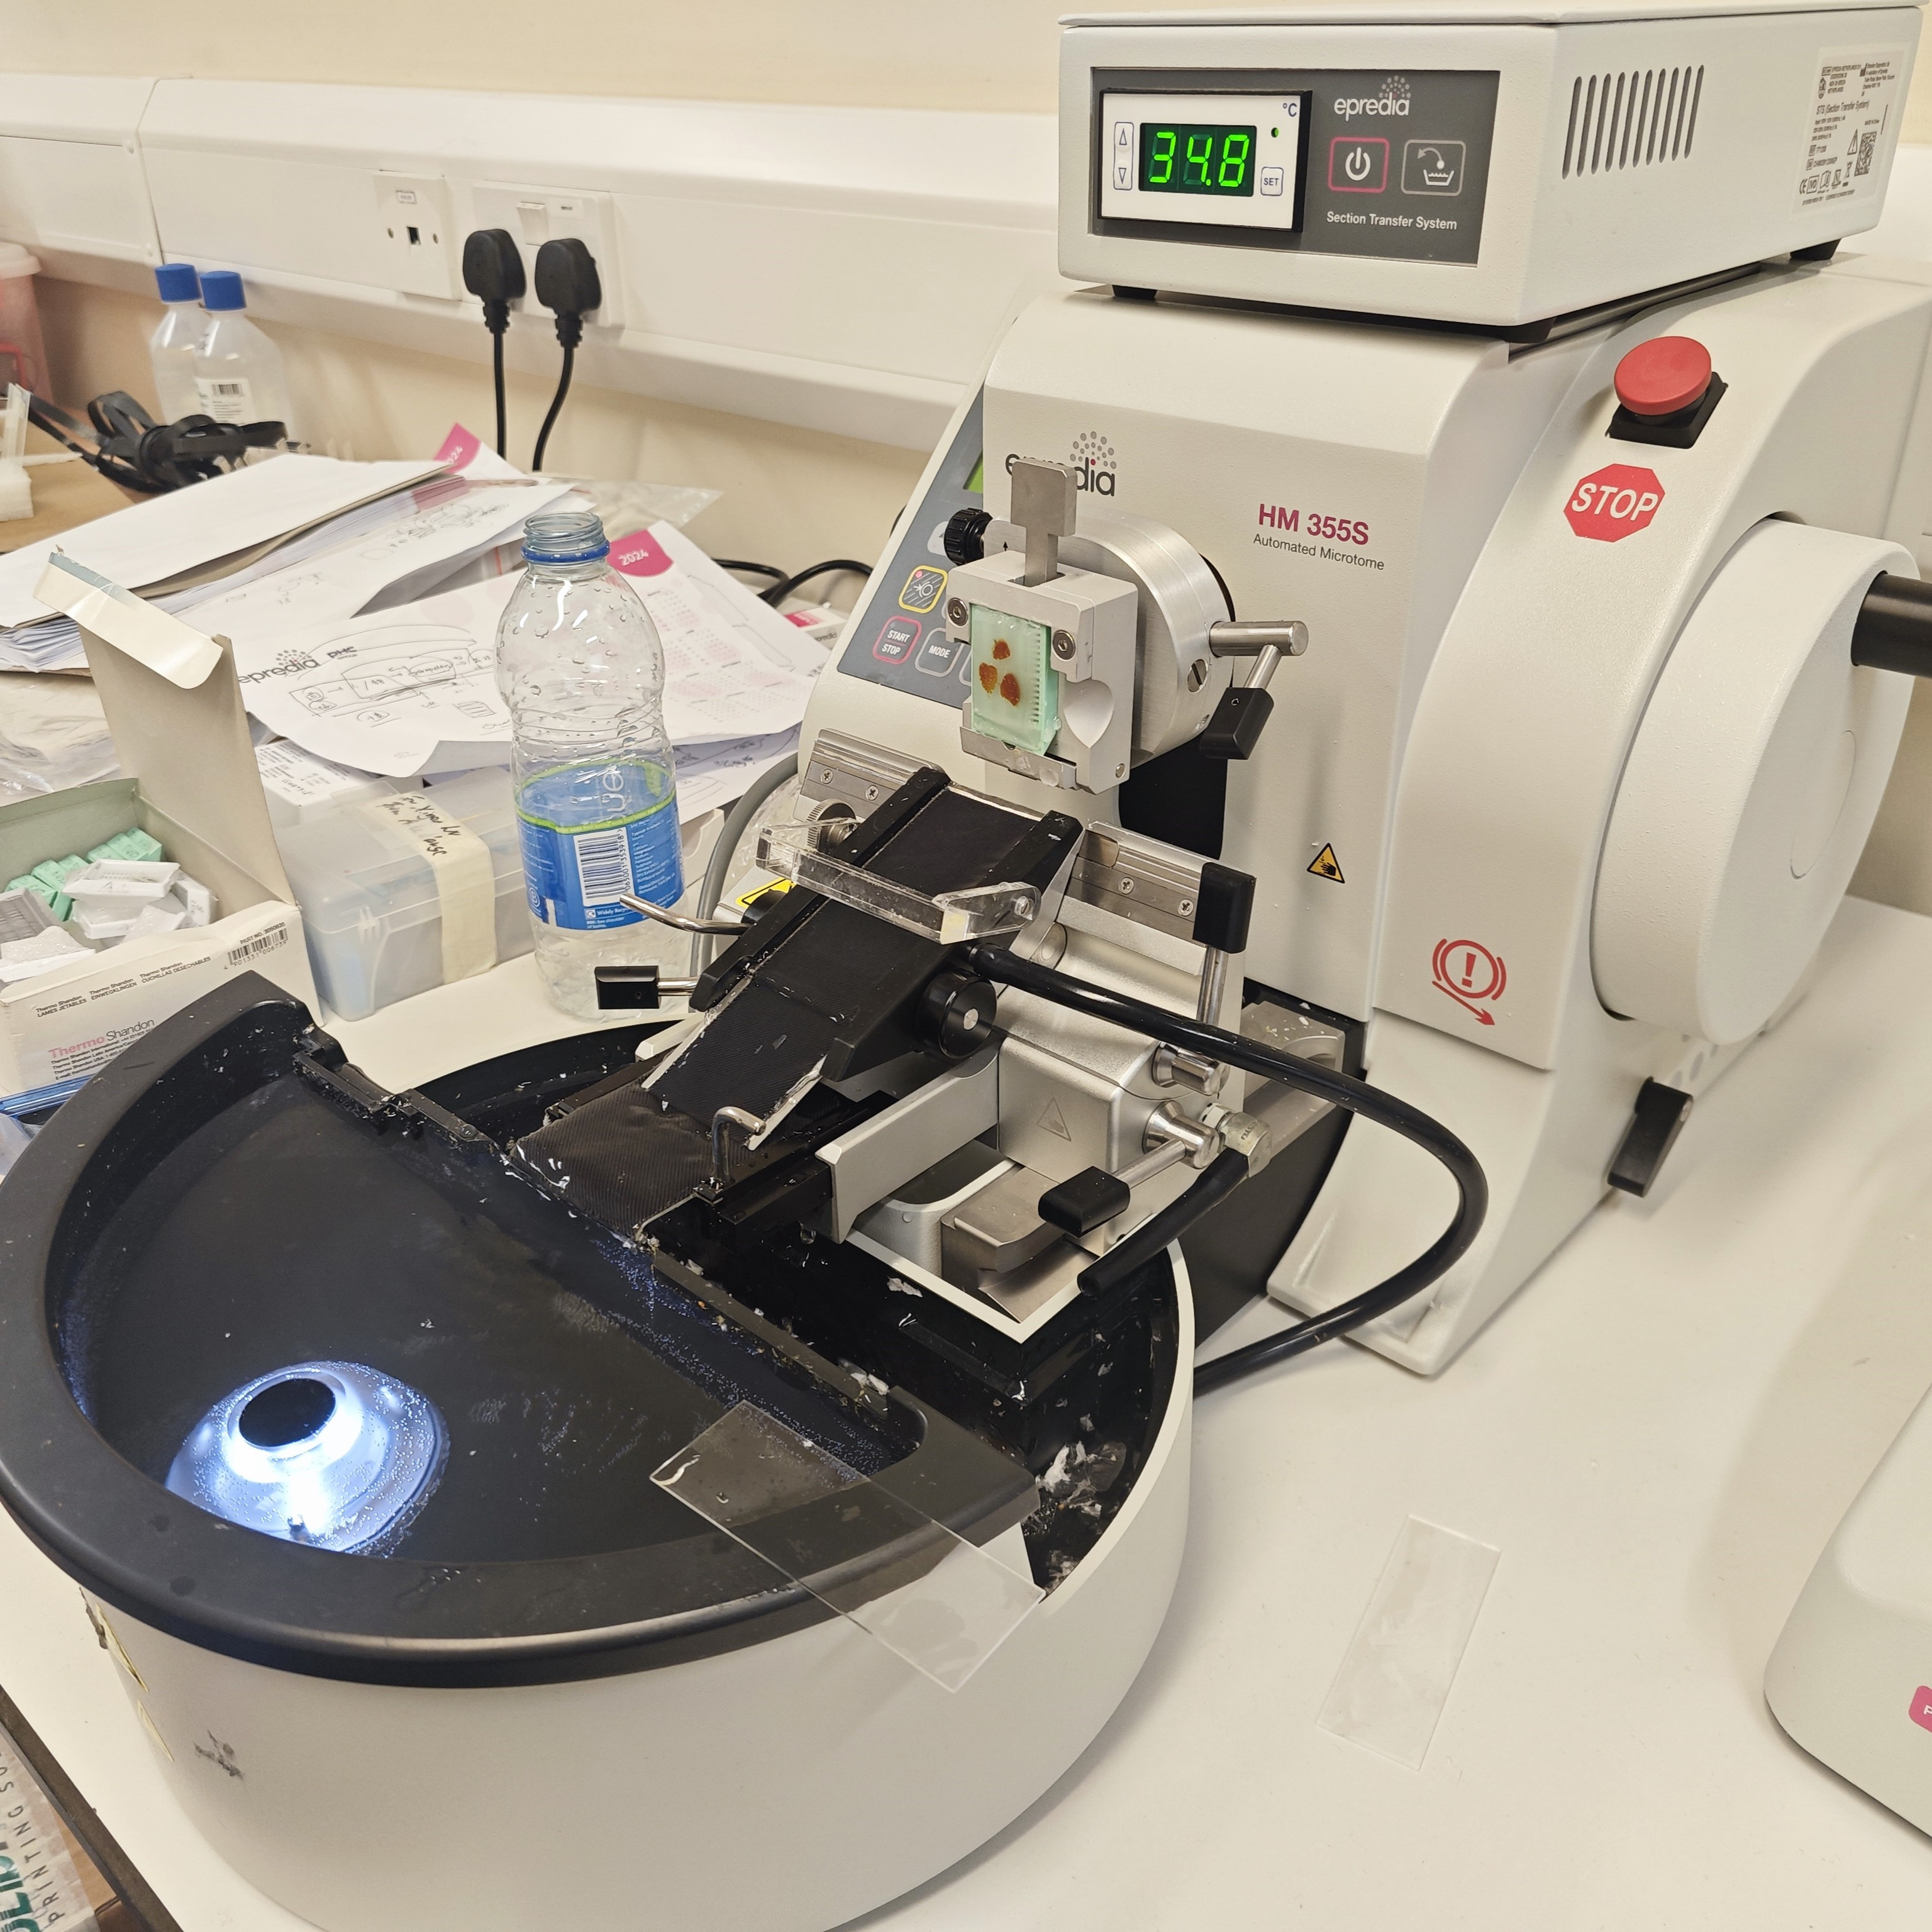
\includegraphics[width=\textwidth]{./fig/machine.jpg}
        \caption{切片机}
        \label{fig:machine}
    \end{minipage}
    \begin{minipage}{0.48\textwidth}
        \centering
        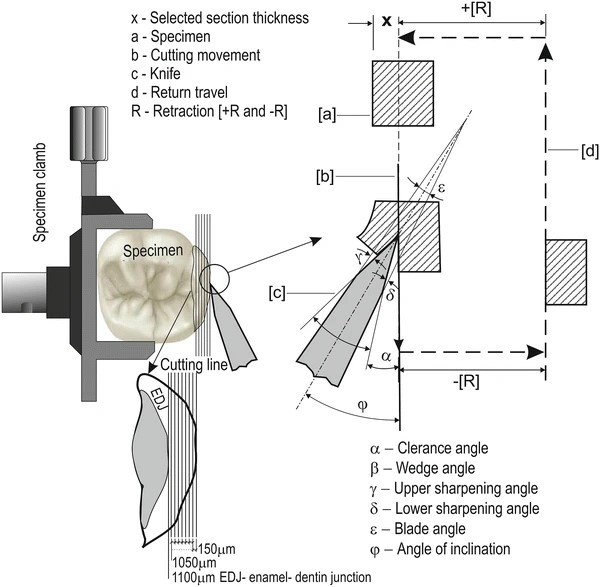
\includegraphics[width=\textwidth]{./fig/10266_2018_353_Fig1_HTML.jpg}
        \caption{切片机示意图}
        \label{fig:cutting_machine}
    \end{minipage}
\end{figure}
% https://link.springer.com/article/10.1007/s10266-018-0353-6


用于切片的生物组织(示例)如\autoref{label:sample}所示

在切削过程中,从切角为8度开始(如\autoref{fig:machine}中的angle of inclination),每次增加0.5度,直到切角为12度。切片机在切片过程中保持给进速度为25,厚度为1。

在切片完成之后,将切好的不同类型的组织切片放在载玻片上(如\autoref{fig:采集样本})所示,待其晾干后转移至VHX7000显微镜下,通过显微镜对每份样品进行拍照,获取到每份样品的电子图像数据(如\autoref{fig:显微镜})。

\begin{figure}[htbp]
    \centering
    \begin{minipage}{0.3\textwidth}
        \centering
        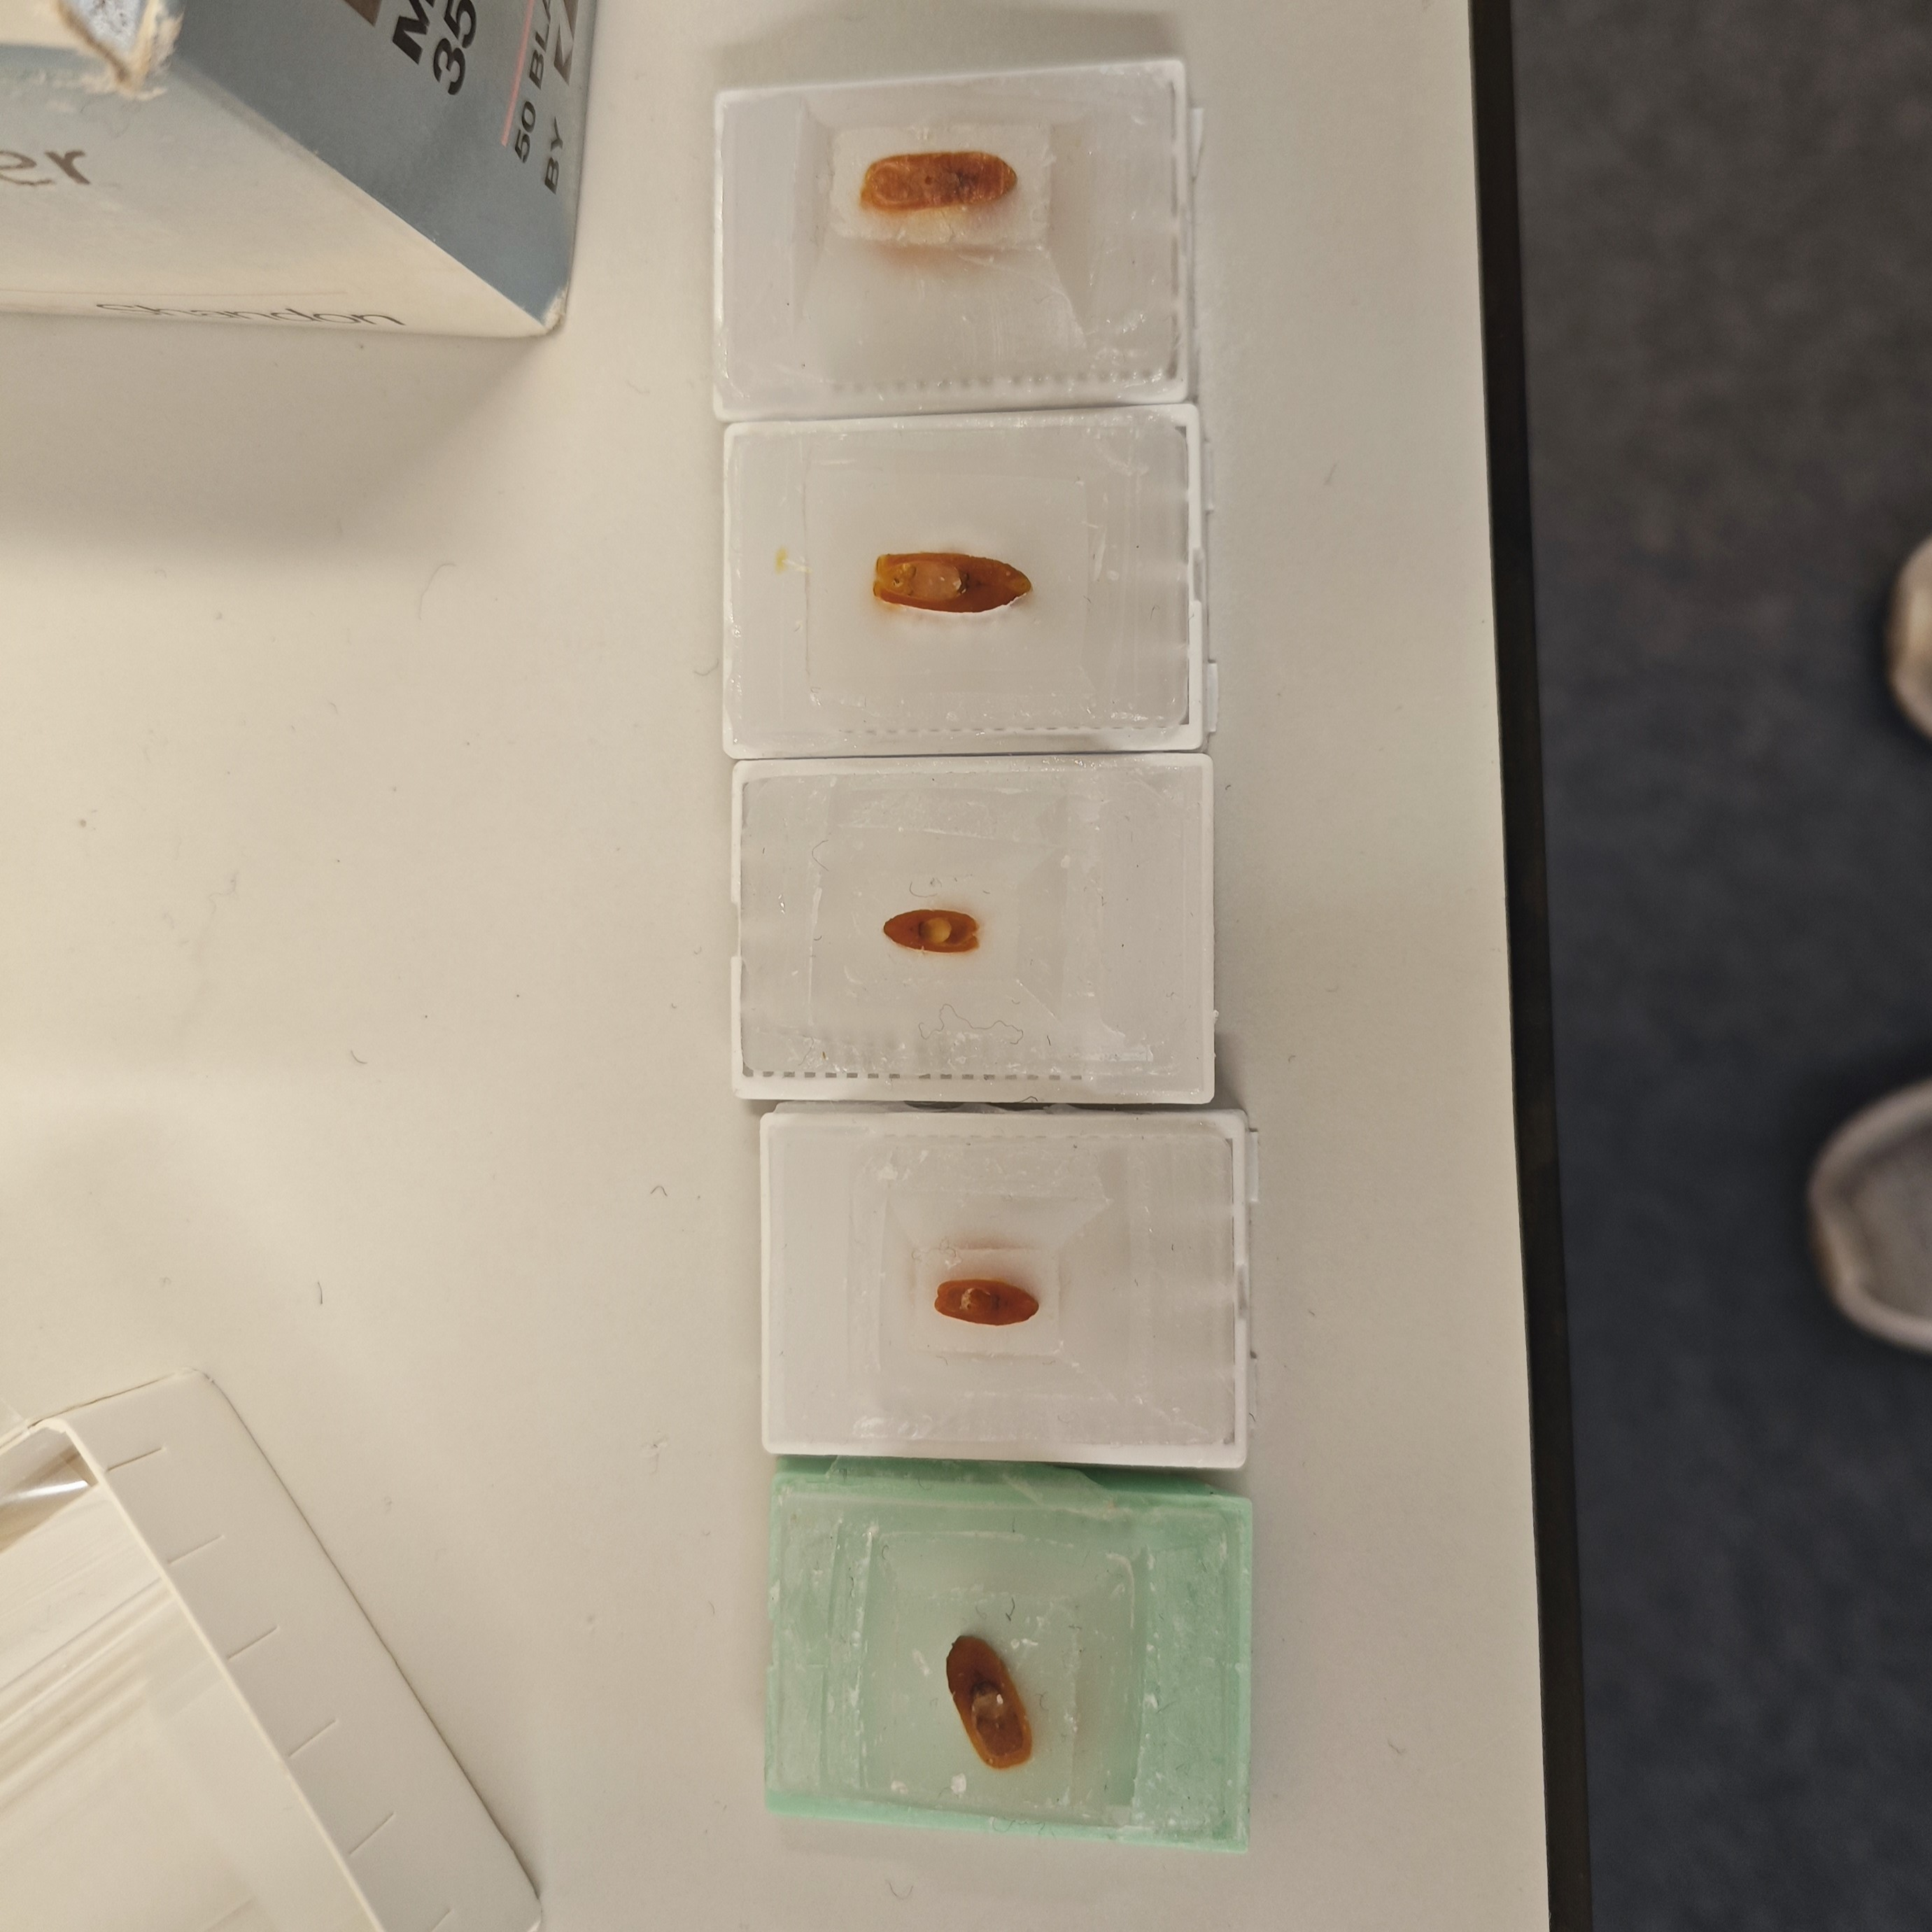
\includegraphics[width=\textwidth]{./fig/sample.jpg}
        \caption{生物组织切片}
        \label{label:sample}
    \end{minipage}
    \begin{minipage}{0.3\textwidth}
        \centering
        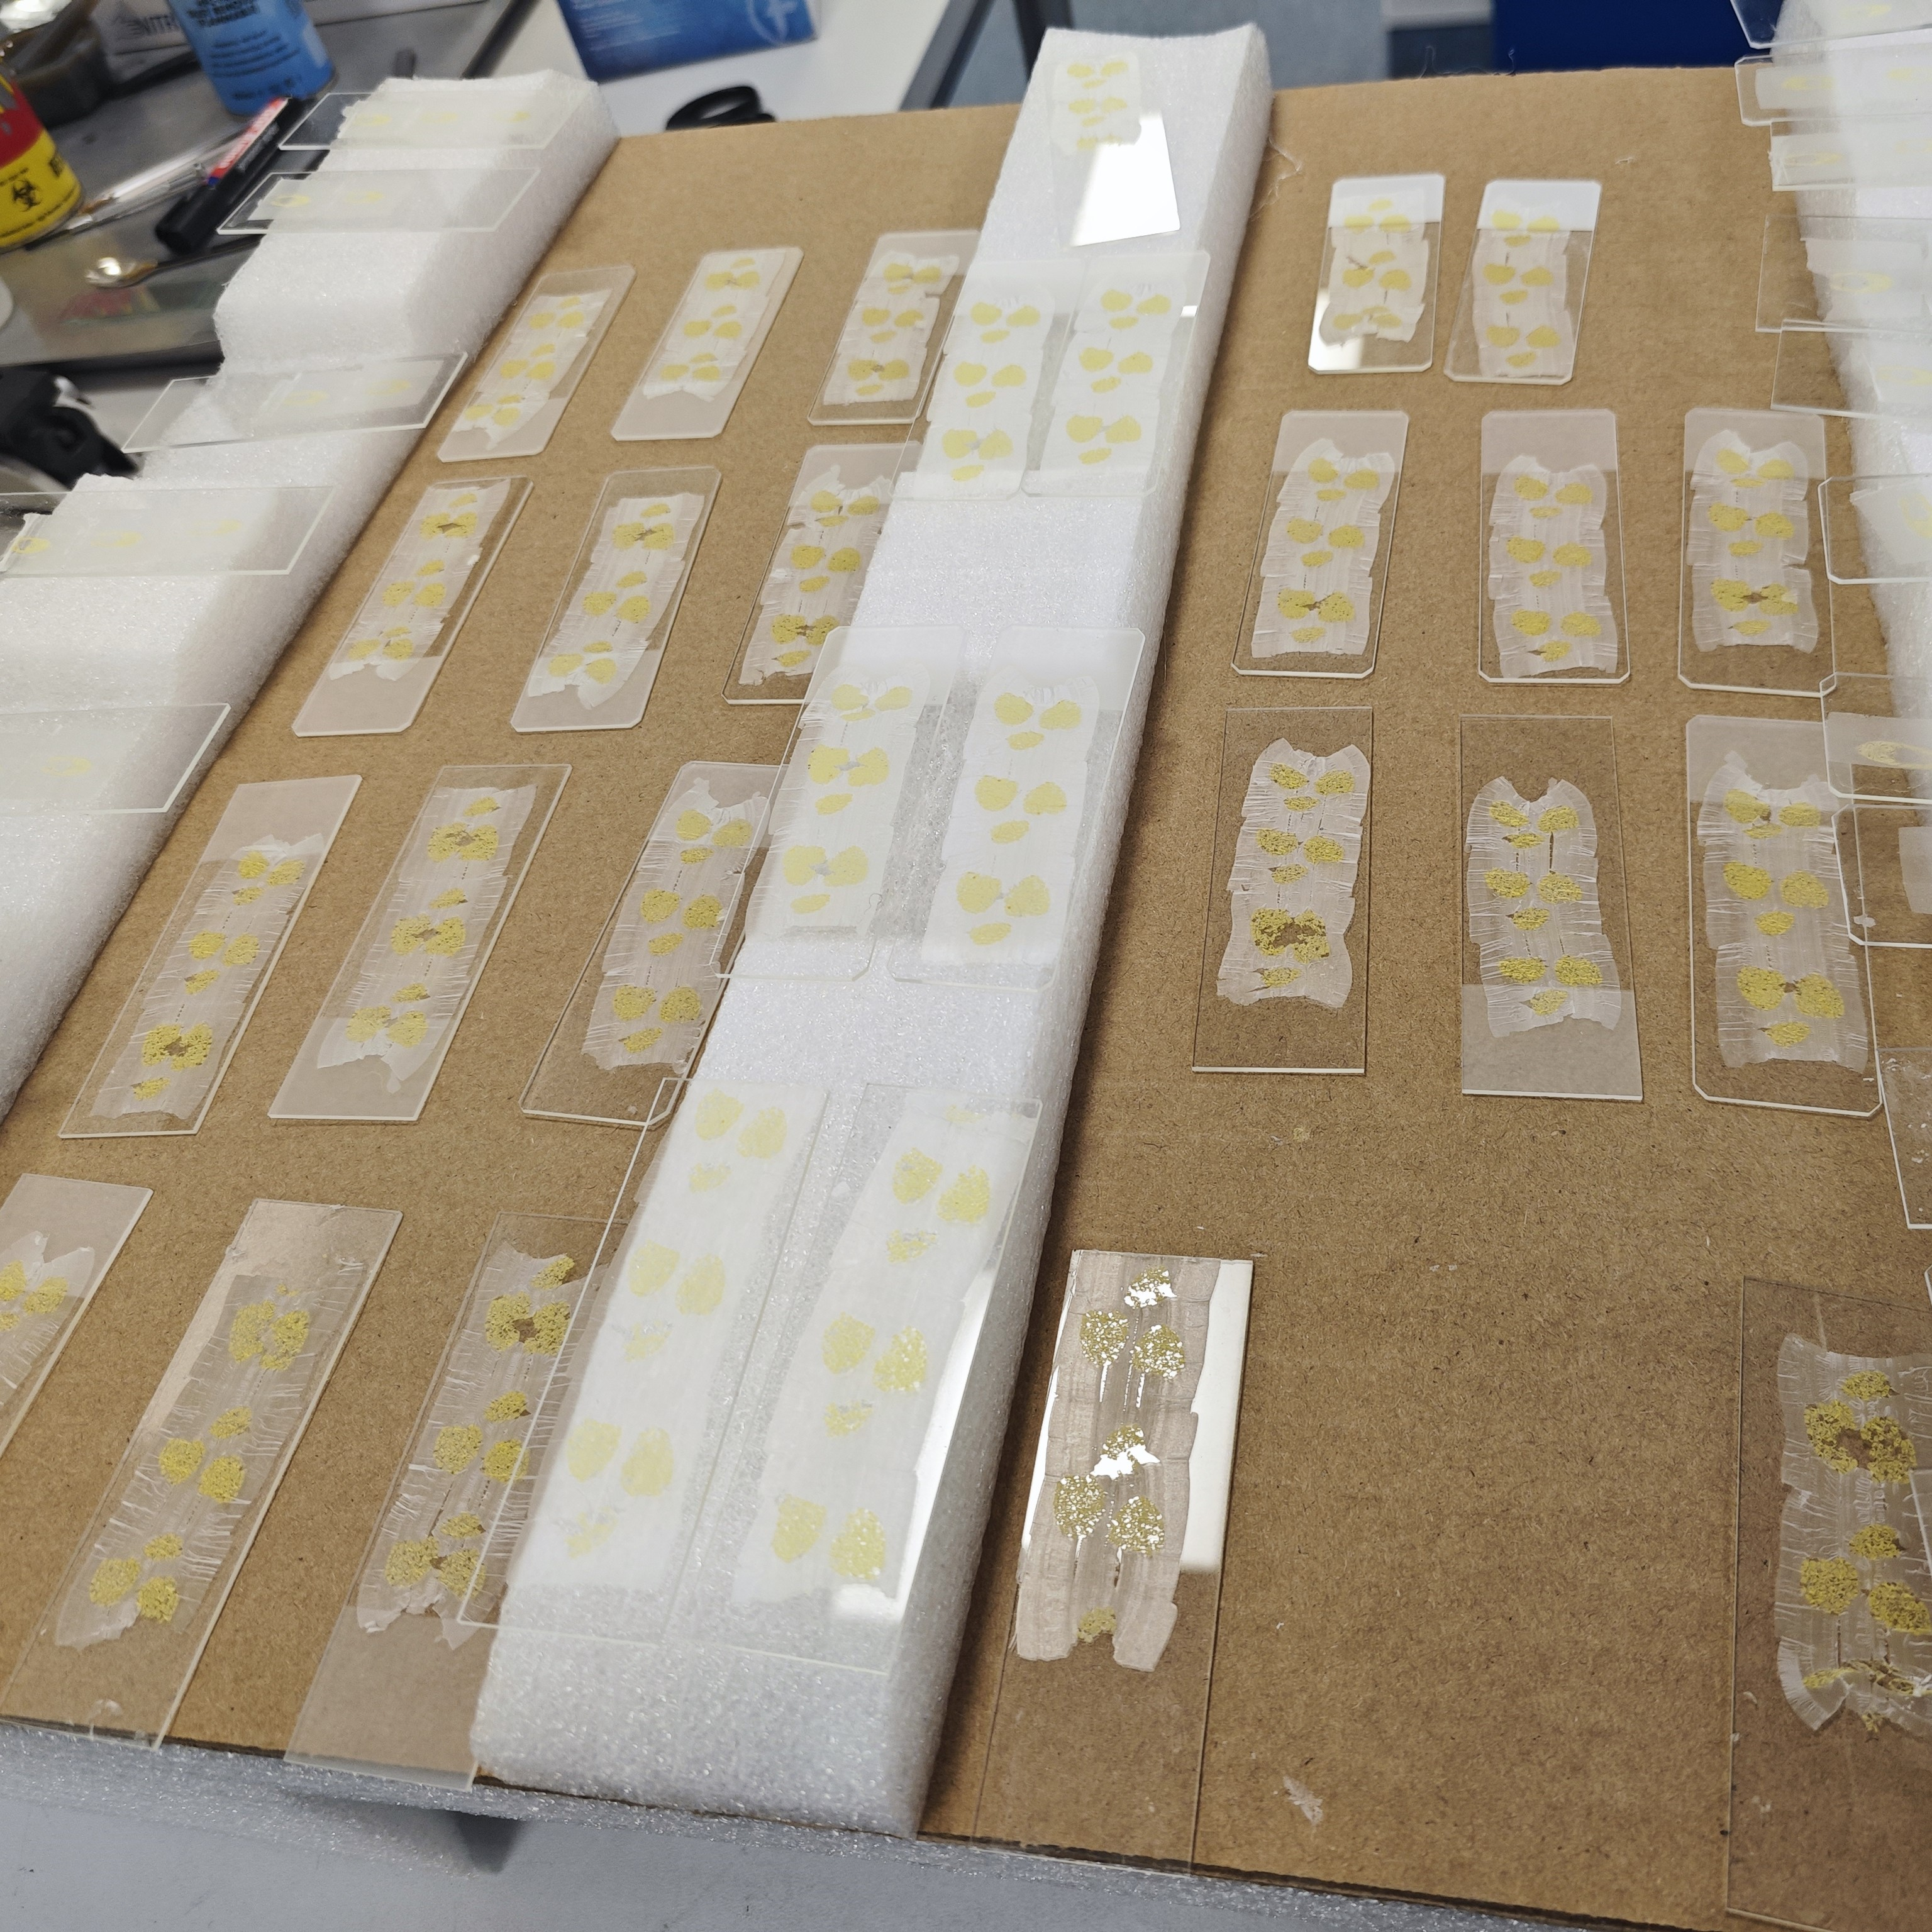
\includegraphics[width=\textwidth]{./fig/采集样本.jpg}
        \caption{采集样本}
        \label{fig:采集样本}
    \end{minipage}
    \begin{minipage}{0.35\textwidth}
        \centering
        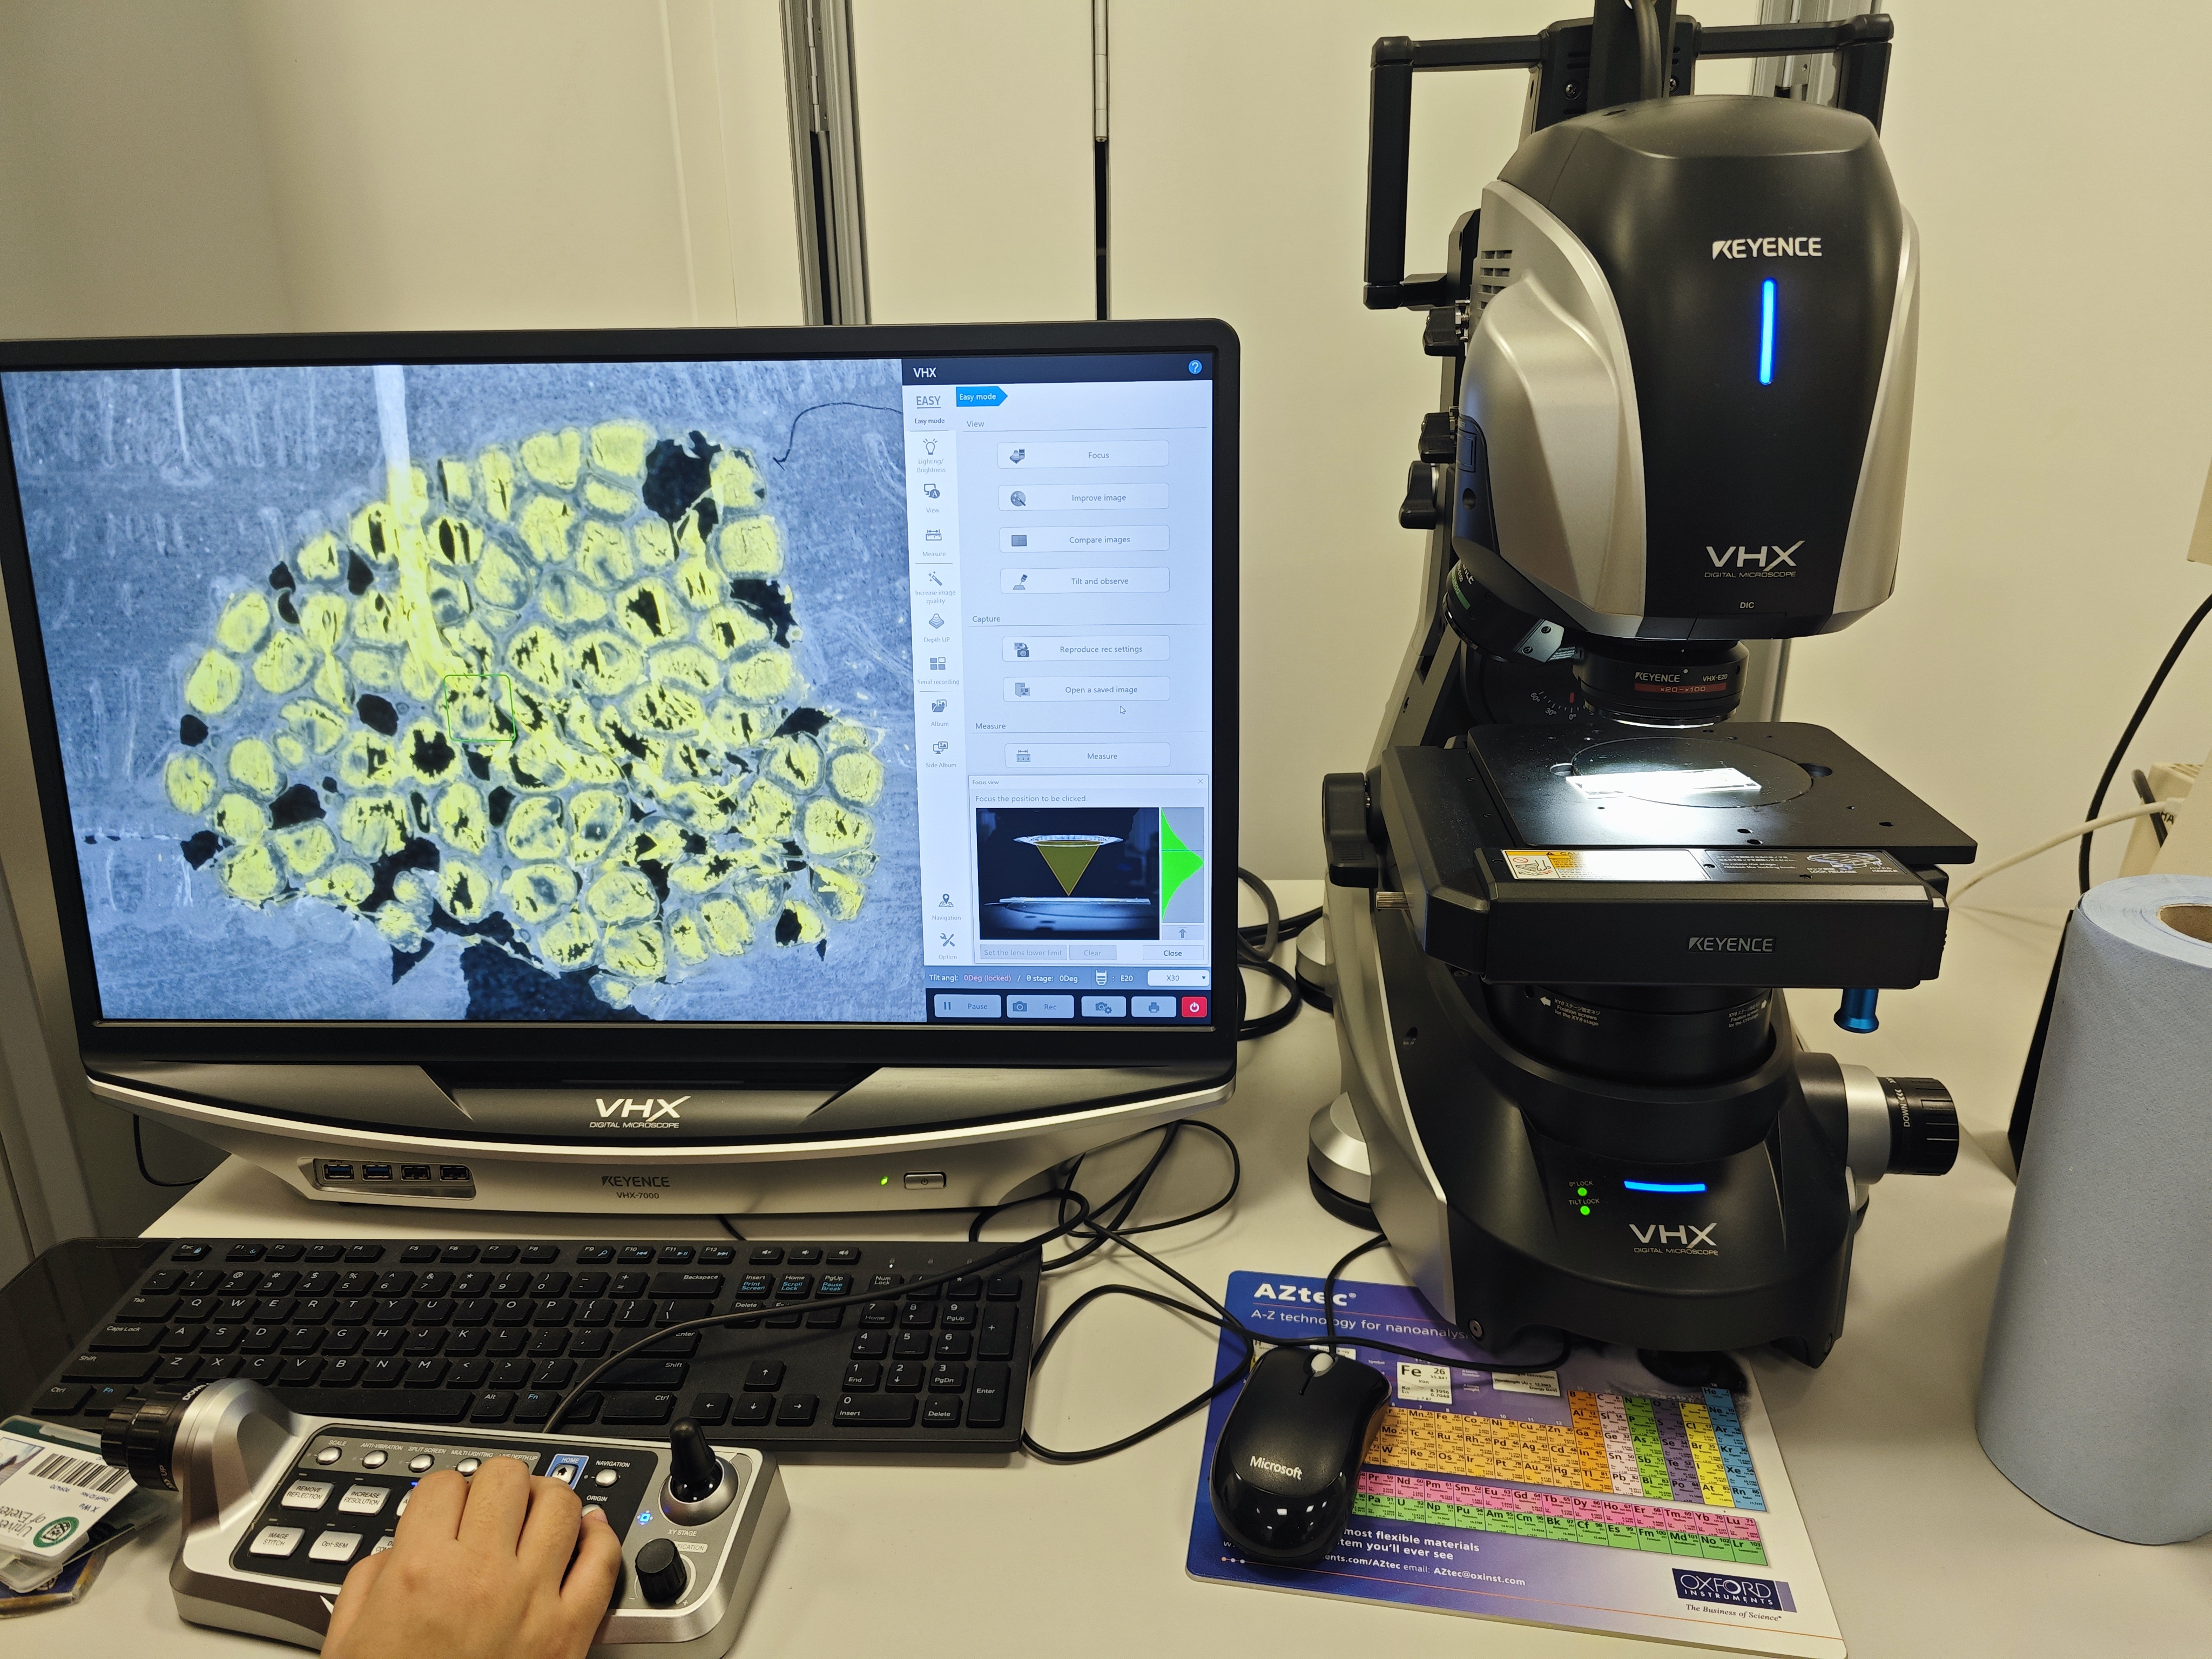
\includegraphics[width=\textwidth]{./fig/显微镜.jpg}
        \caption{显微镜}
        \label{fig:显微镜}
    \end{minipage}
\end{figure}

%图片需要后续更改为卵巢的

据此,一共得到9组数据,代表了从8到12每0.5度切角的数据。一共得到约为200张图片,每张图片的分辨率为2880*2160。其中一张(切角9.5度)如\autoref{fig:sample9.5}所示。

\begin{figure}
    \centering
    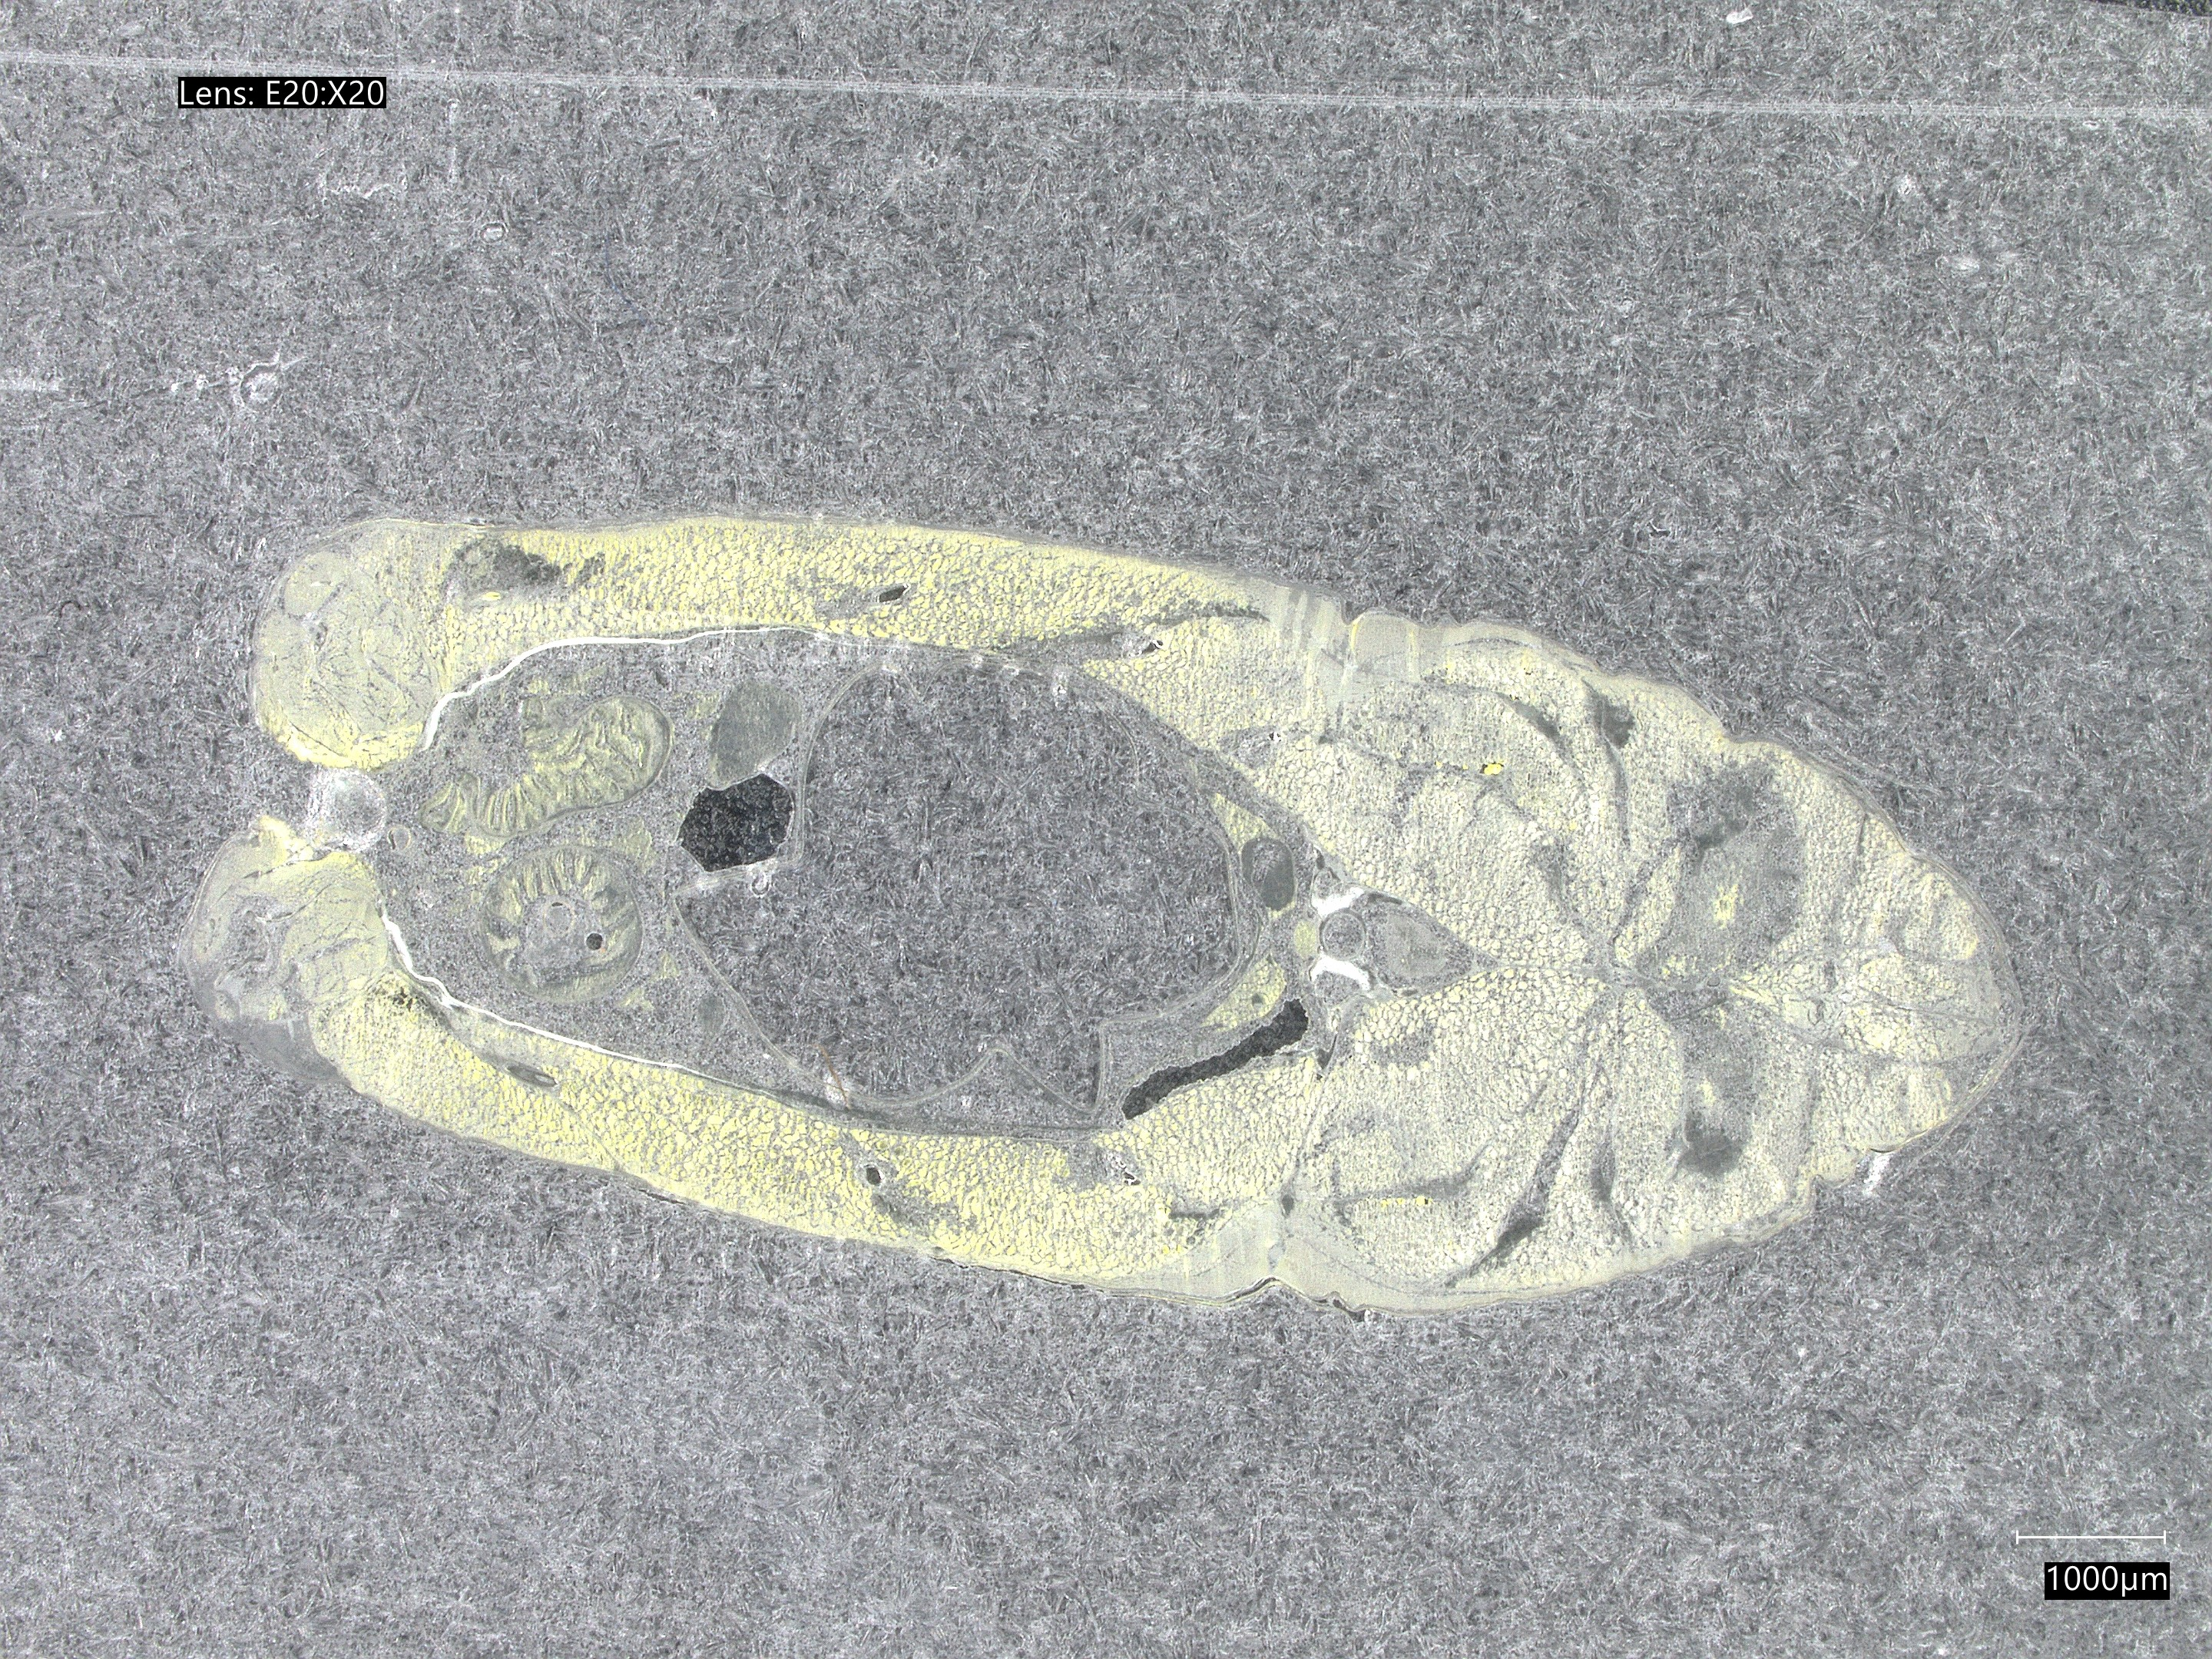
\includegraphics[width=0.8\textwidth]{./fig/sample9.5.jpg}
    \caption{切角9.5度的样本}
    \label{fig:sample9.5}
\end{figure}

对于这9组数据,需要找到的是在何种切角下,生物组织的完整度最高(质量最好)。因此现在需要将这9组数据根据生物组织的完整度进行重新标注。

根据刀片切割对生物组织的影响,我们将生物组织的完整度分为五个类别,分别为:horizental line, vertical line, slope, other, normal。其中horizental line代表显著的以水平白线为瑕疵的样本,vertical line代表显著的以竖直白线为瑕疵的样本,slope代表图像采集中存在明显的角度(不利于观察),other代表其他瑕疵(如采集中存在明暗显著差别的色块),normal代表正常的生物组织样本。这五类标签的示例图片如下所示。

\begin{figure}
    \centering
    \begin{minipage}{0.45\textwidth}
        \centering
        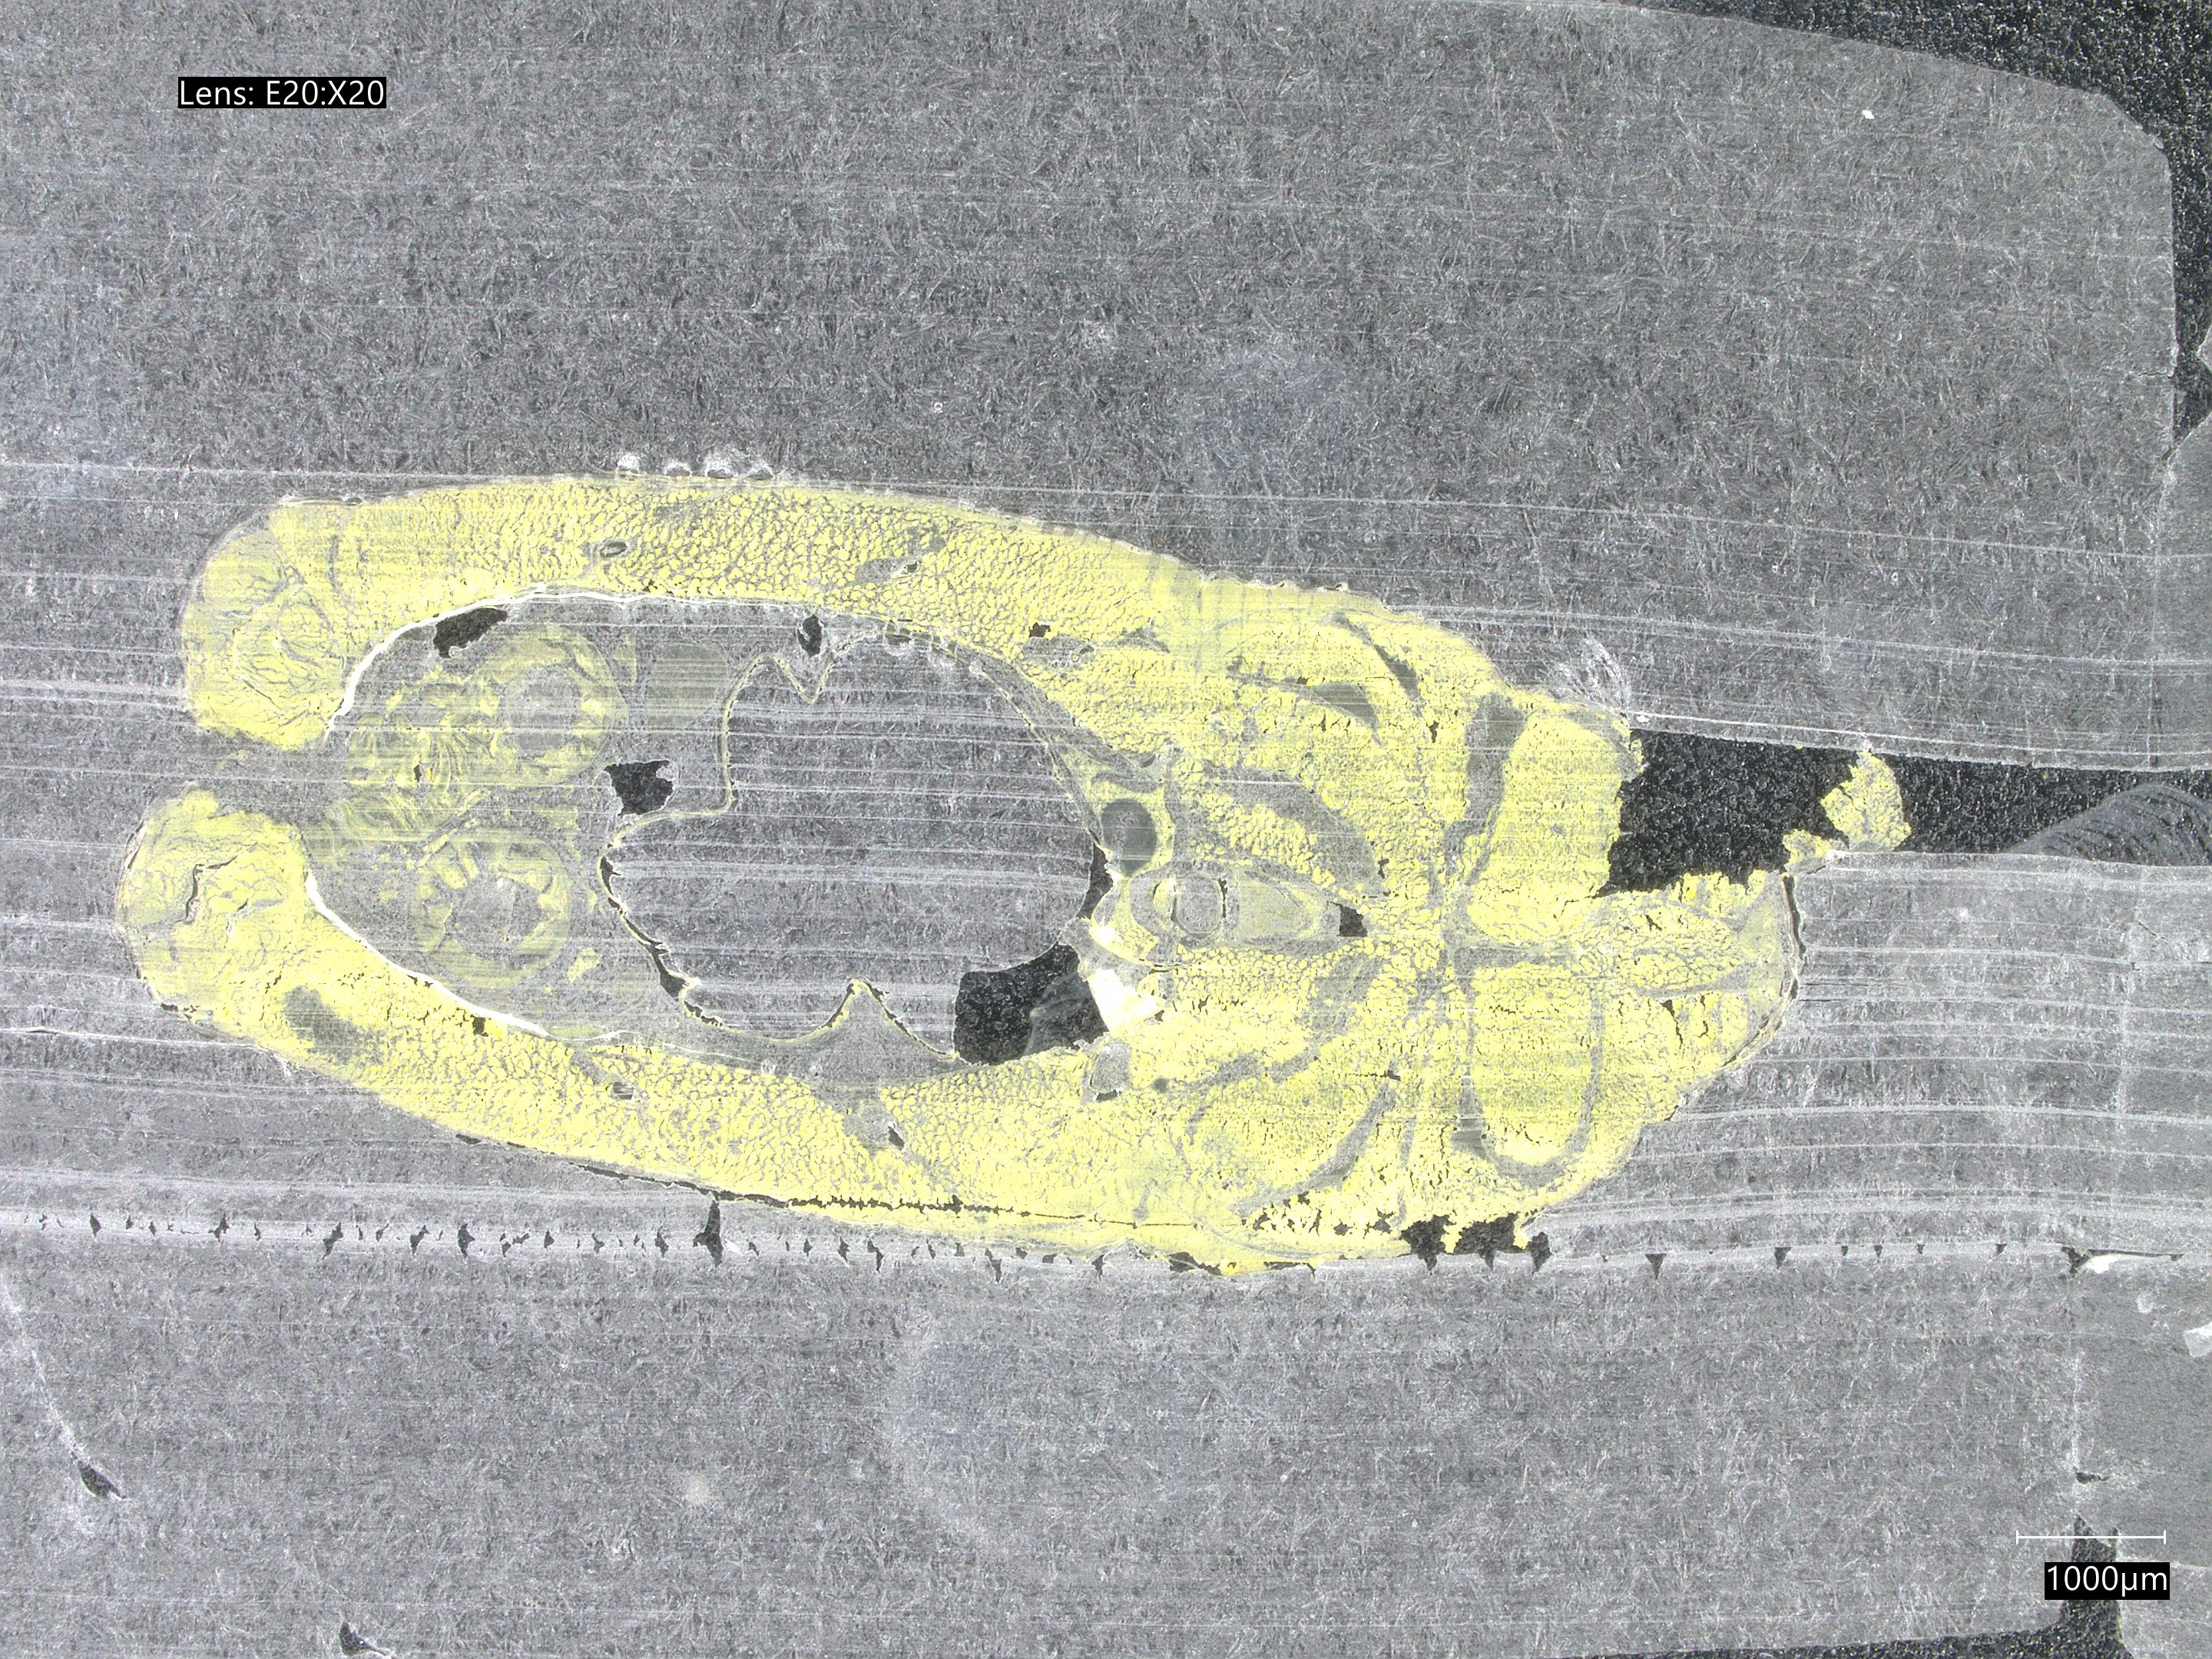
\includegraphics[width=\textwidth]{./fig/sample_1/horizental_line.jpg}
        \caption{horizental line}
        \label{fig:horizental_line}
    \end{minipage}
    \begin{minipage}{0.45\textwidth}
        \centering
        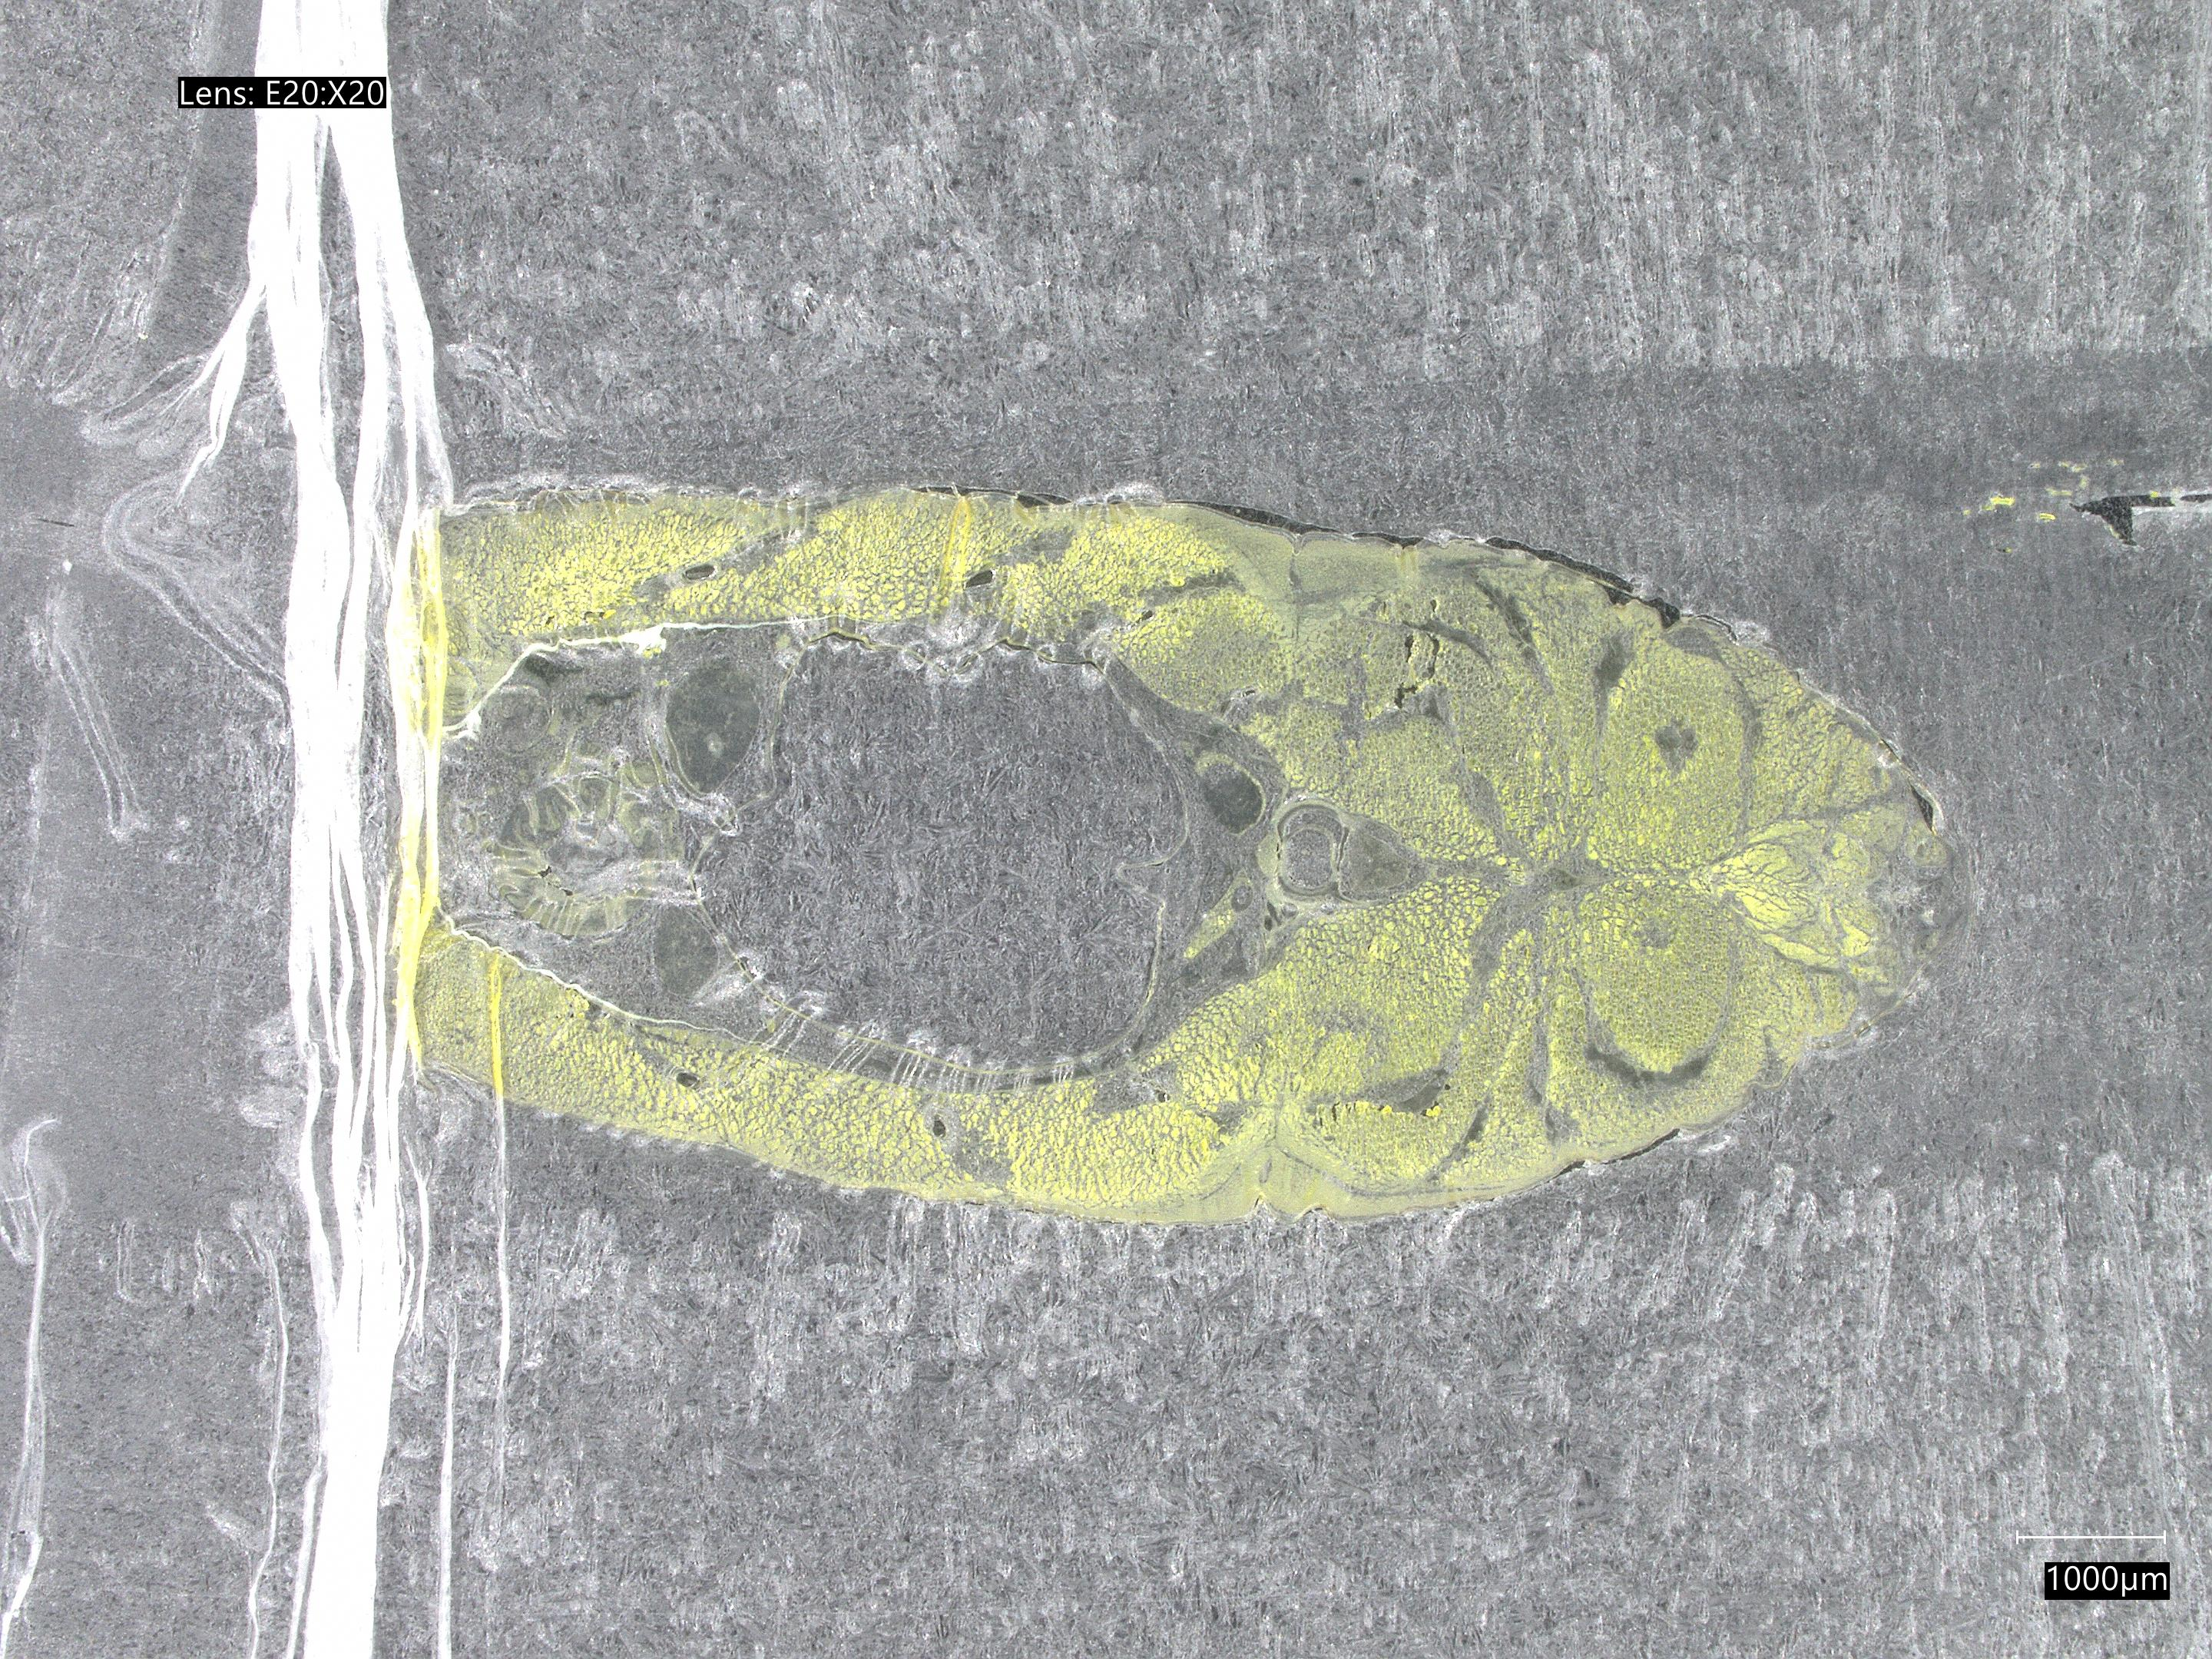
\includegraphics[width=\textwidth]{./fig/sample_1/vertical_line.jpg}
        \caption{vertical line}
        \label{fig:vertical_line}
    \end{minipage}
\end{figure}

\begin{figure}
    \centering
    \begin{minipage}{0.45\textwidth}
        \centering
        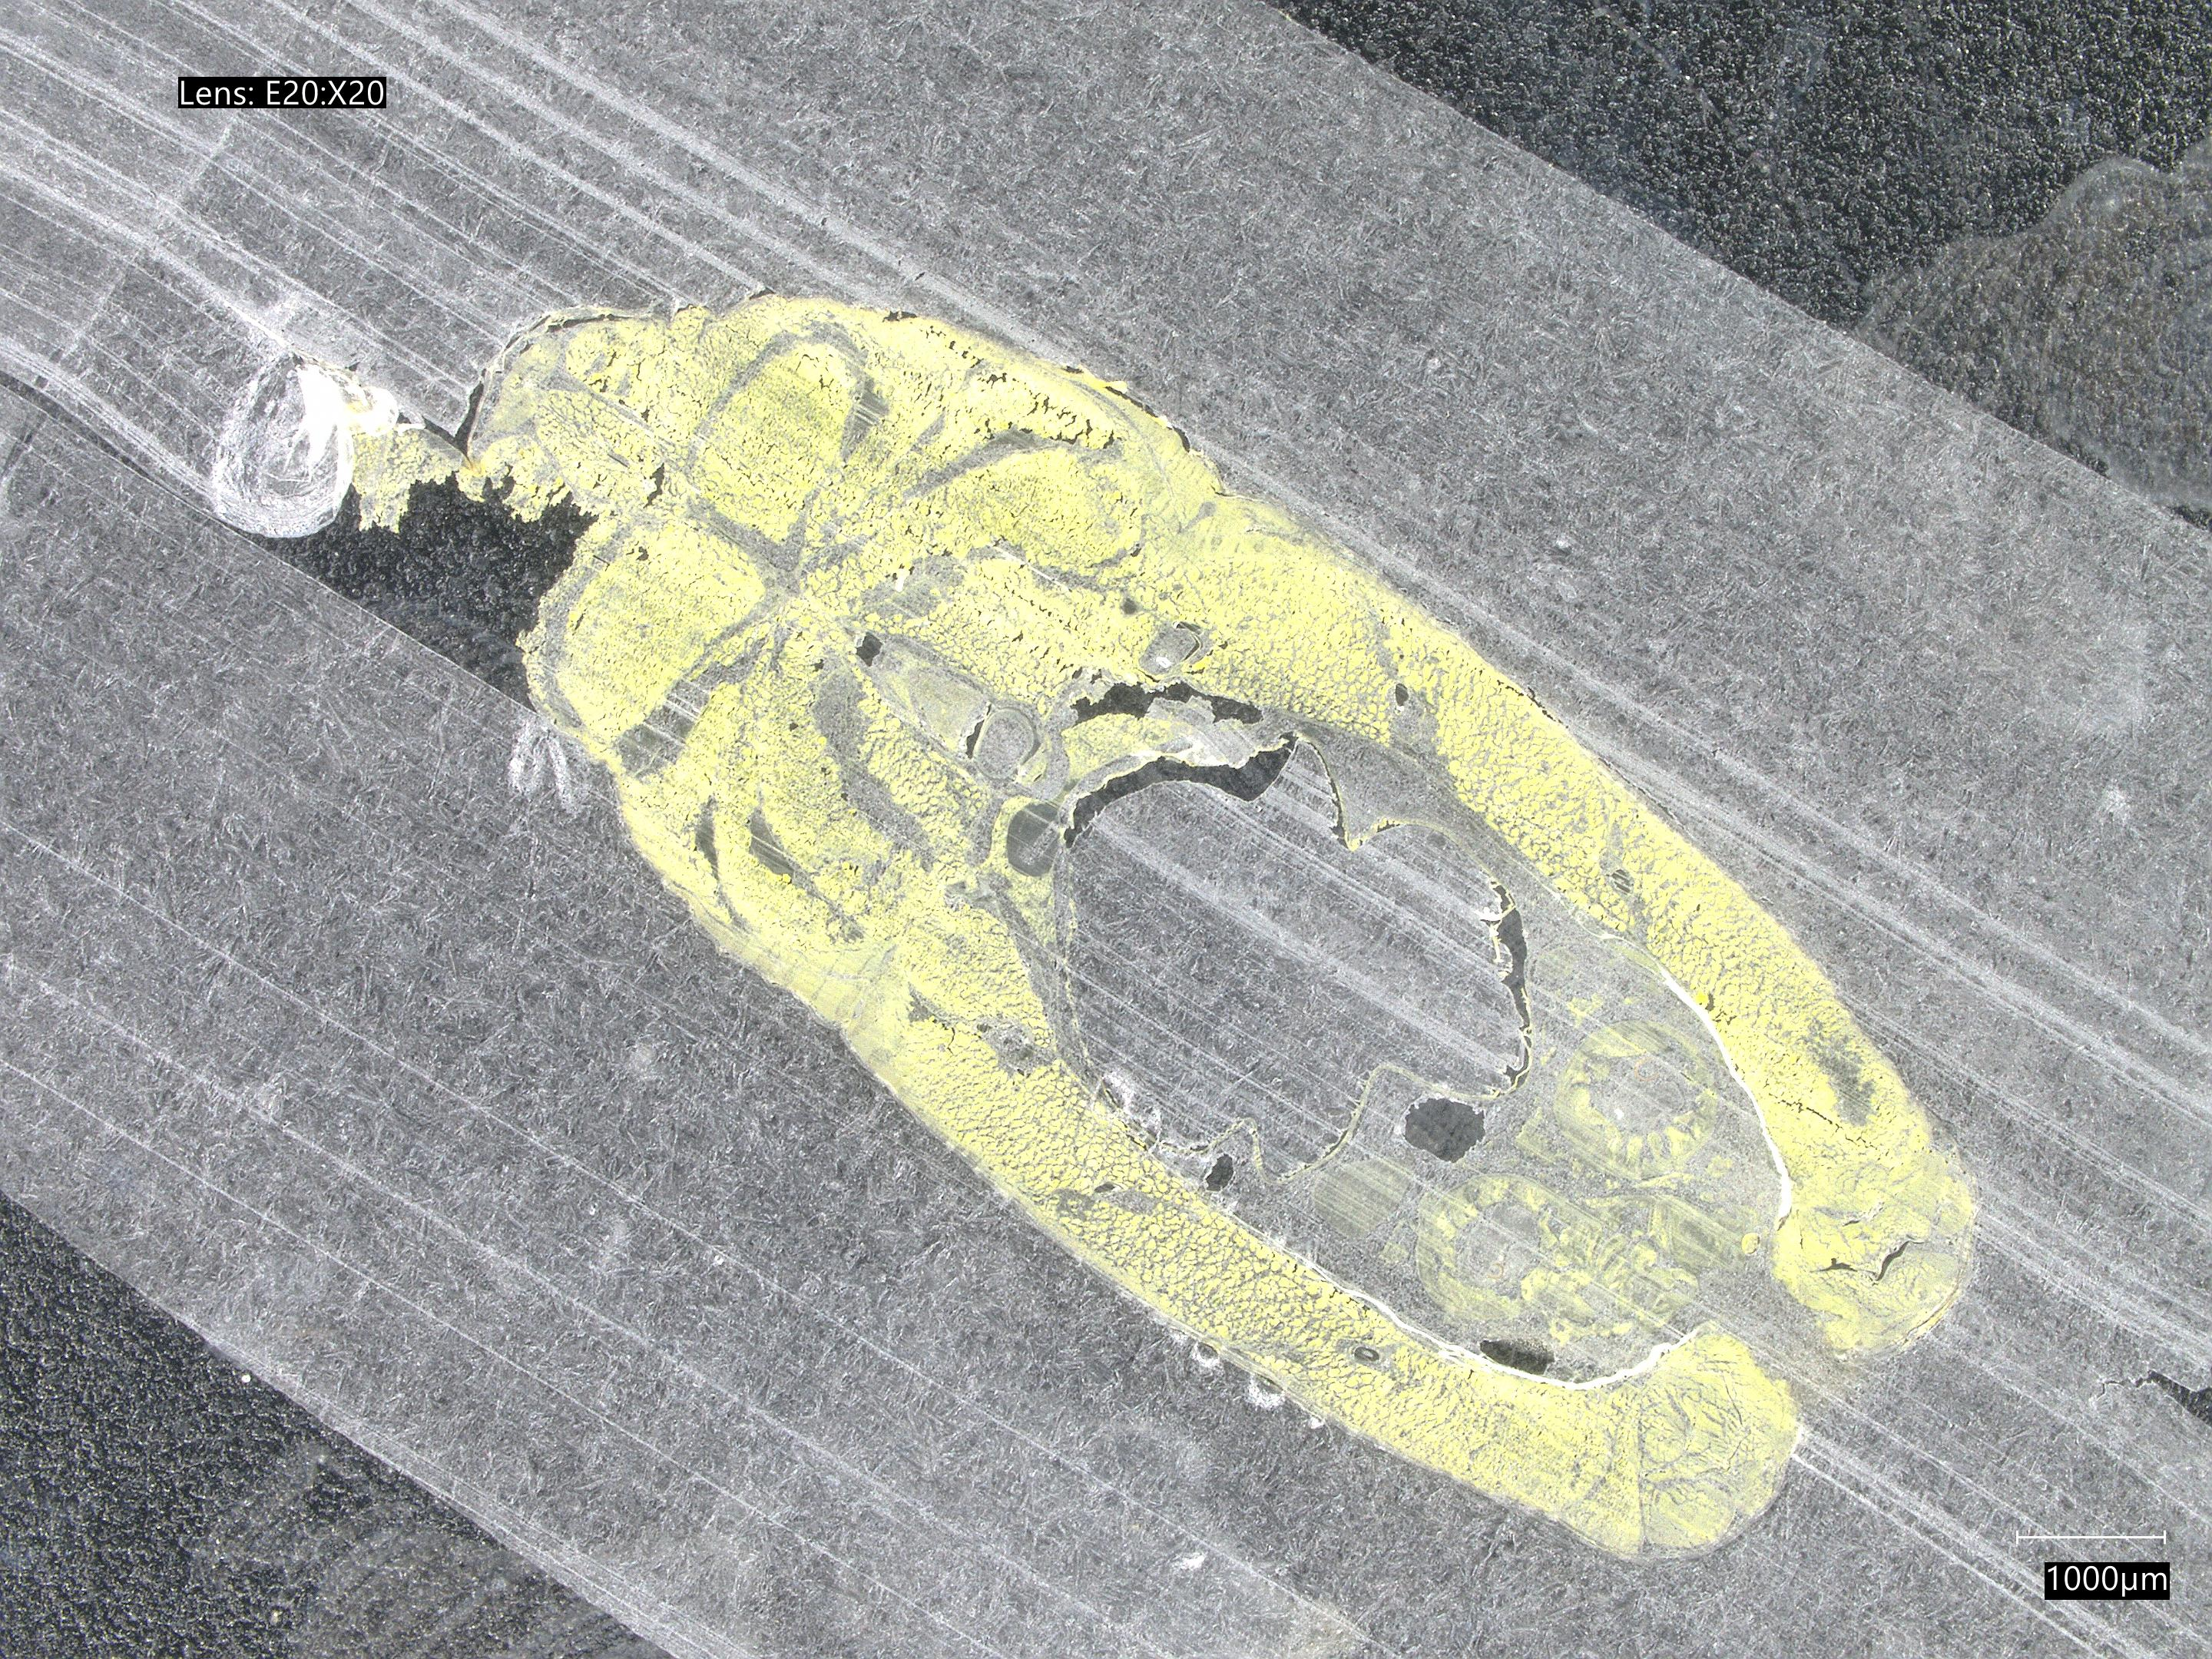
\includegraphics[width=\textwidth]{./fig/sample_1/slope.jpg}
        \caption{slope}
        \label{fig:slope}
    \end{minipage}
    \begin{minipage}{0.45\textwidth}
        \centering
        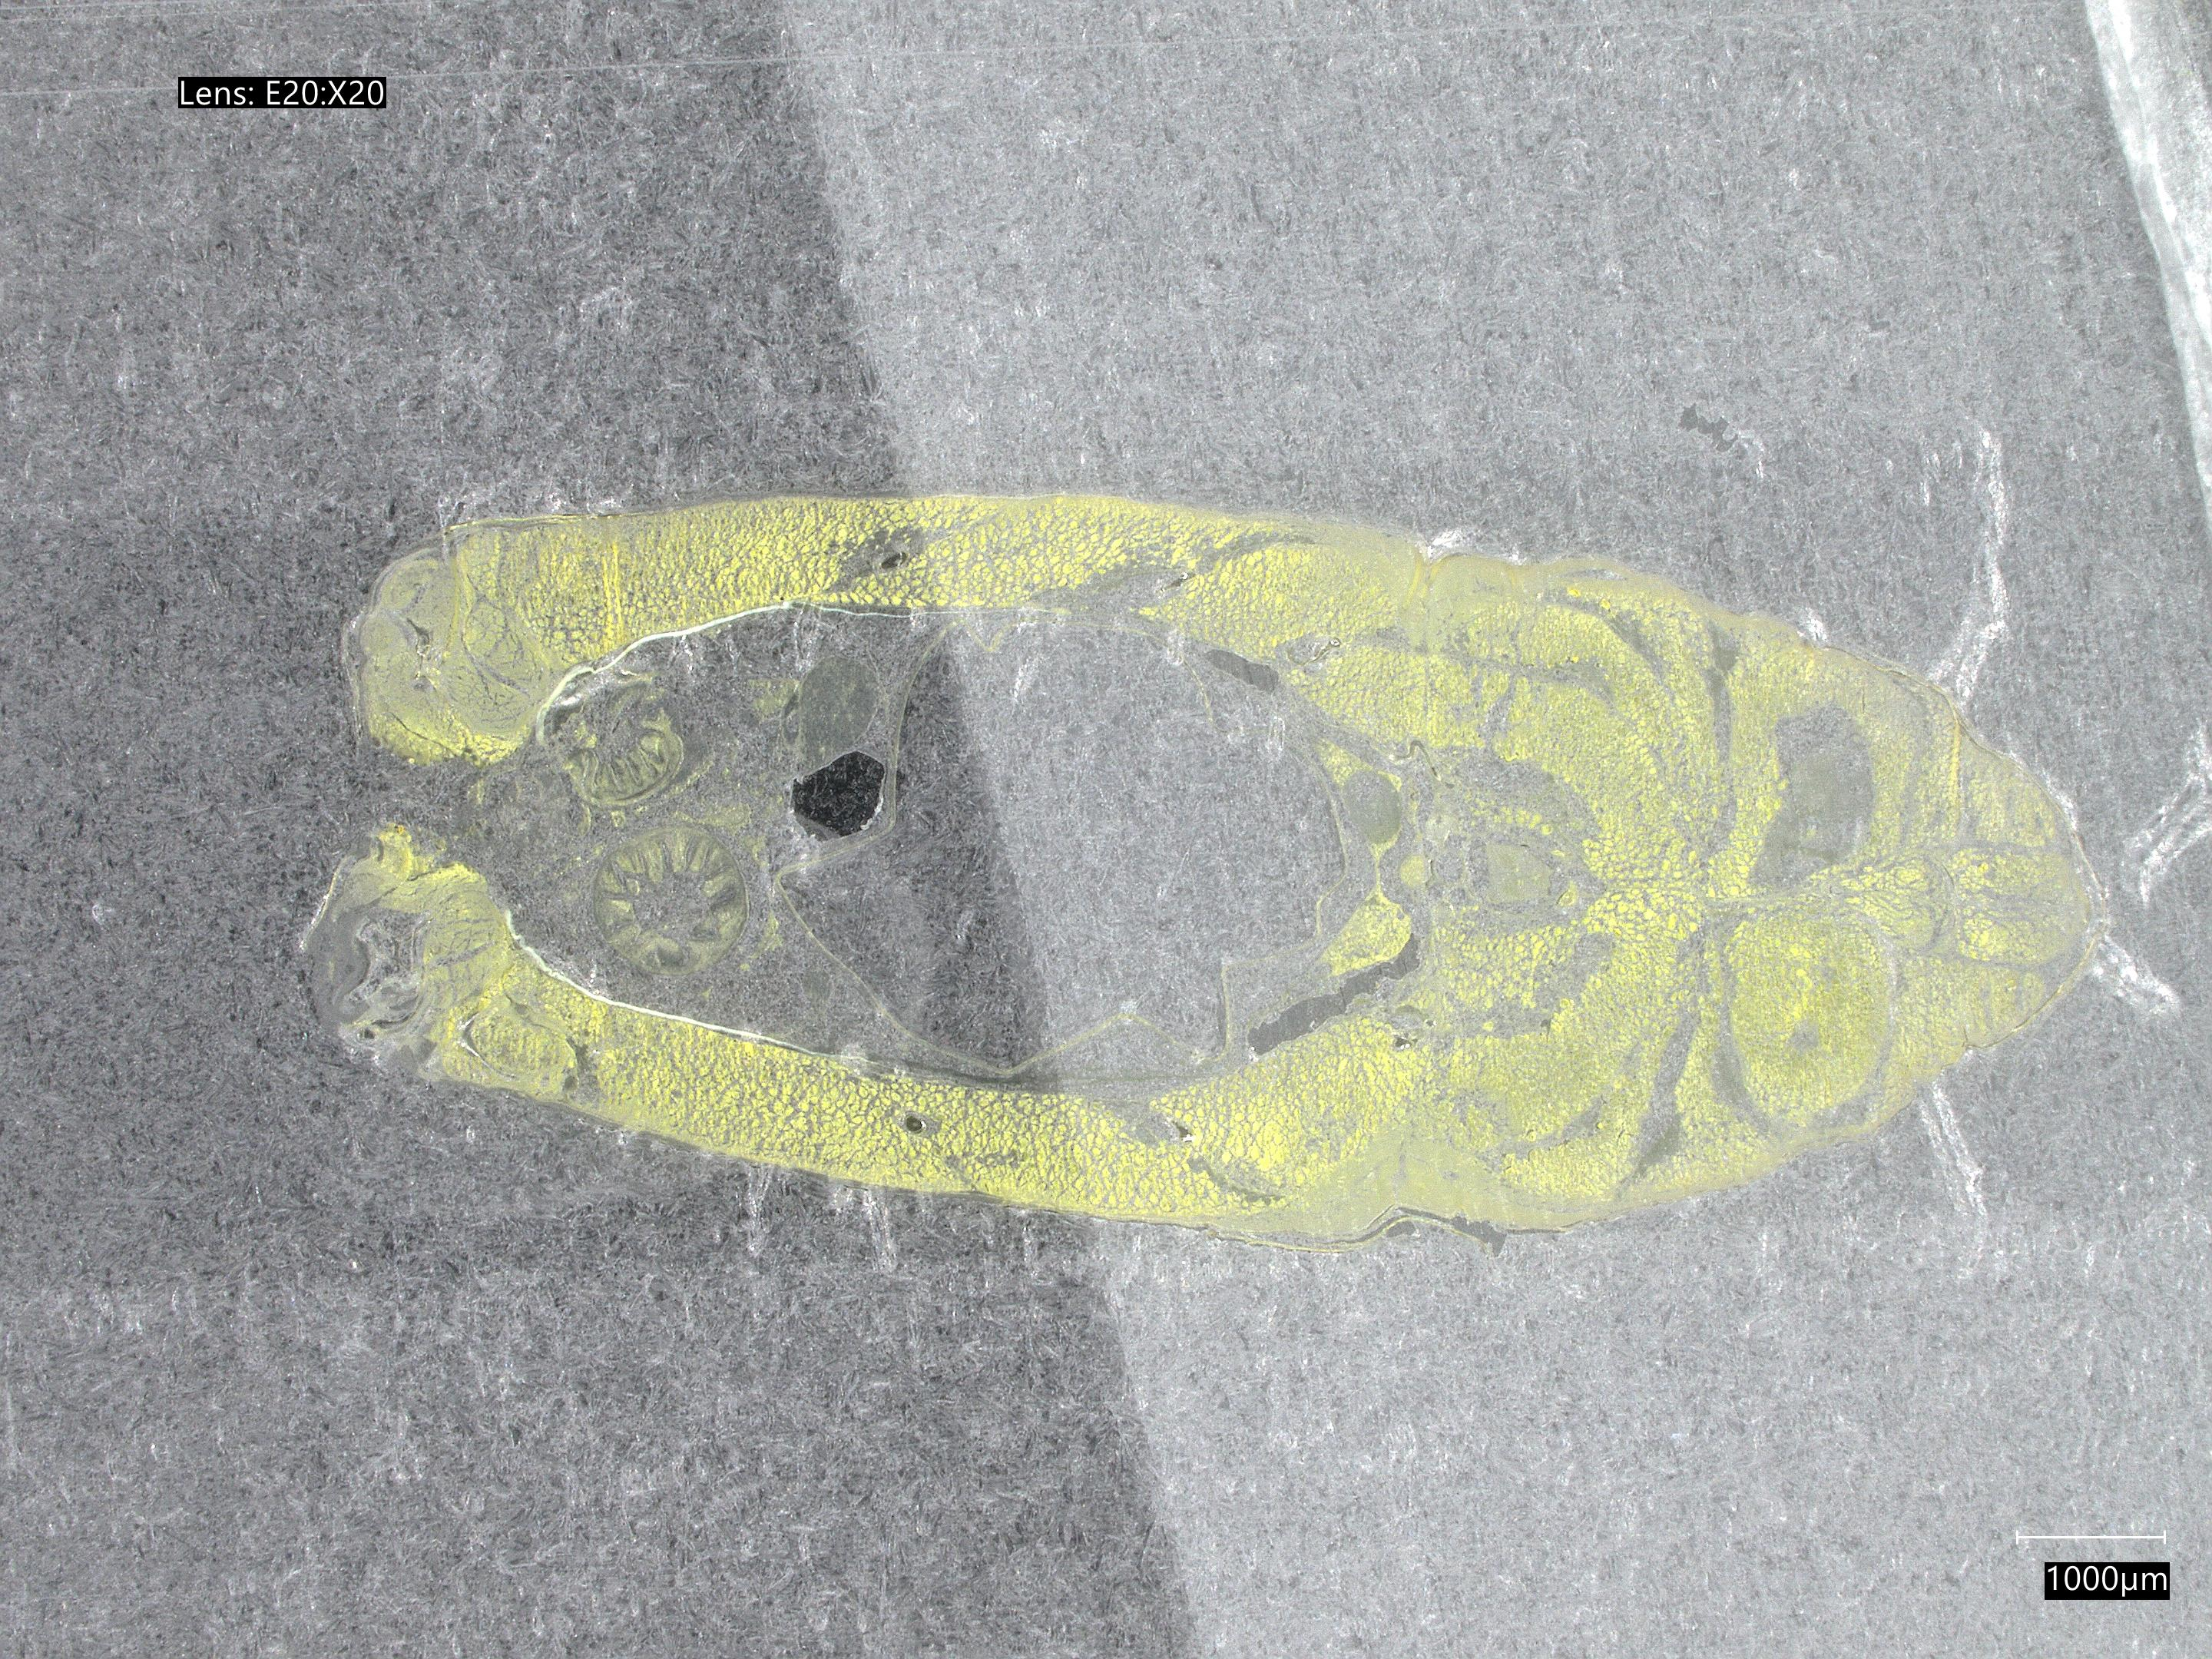
\includegraphics[width=\textwidth]{./fig/sample_1/other.jpg}
        \caption{other}
        \label{fig:other}
    \end{minipage}
\end{figure}

\begin{figure}
    \centering
    \begin{minipage}{0.45\textwidth}
        \centering
        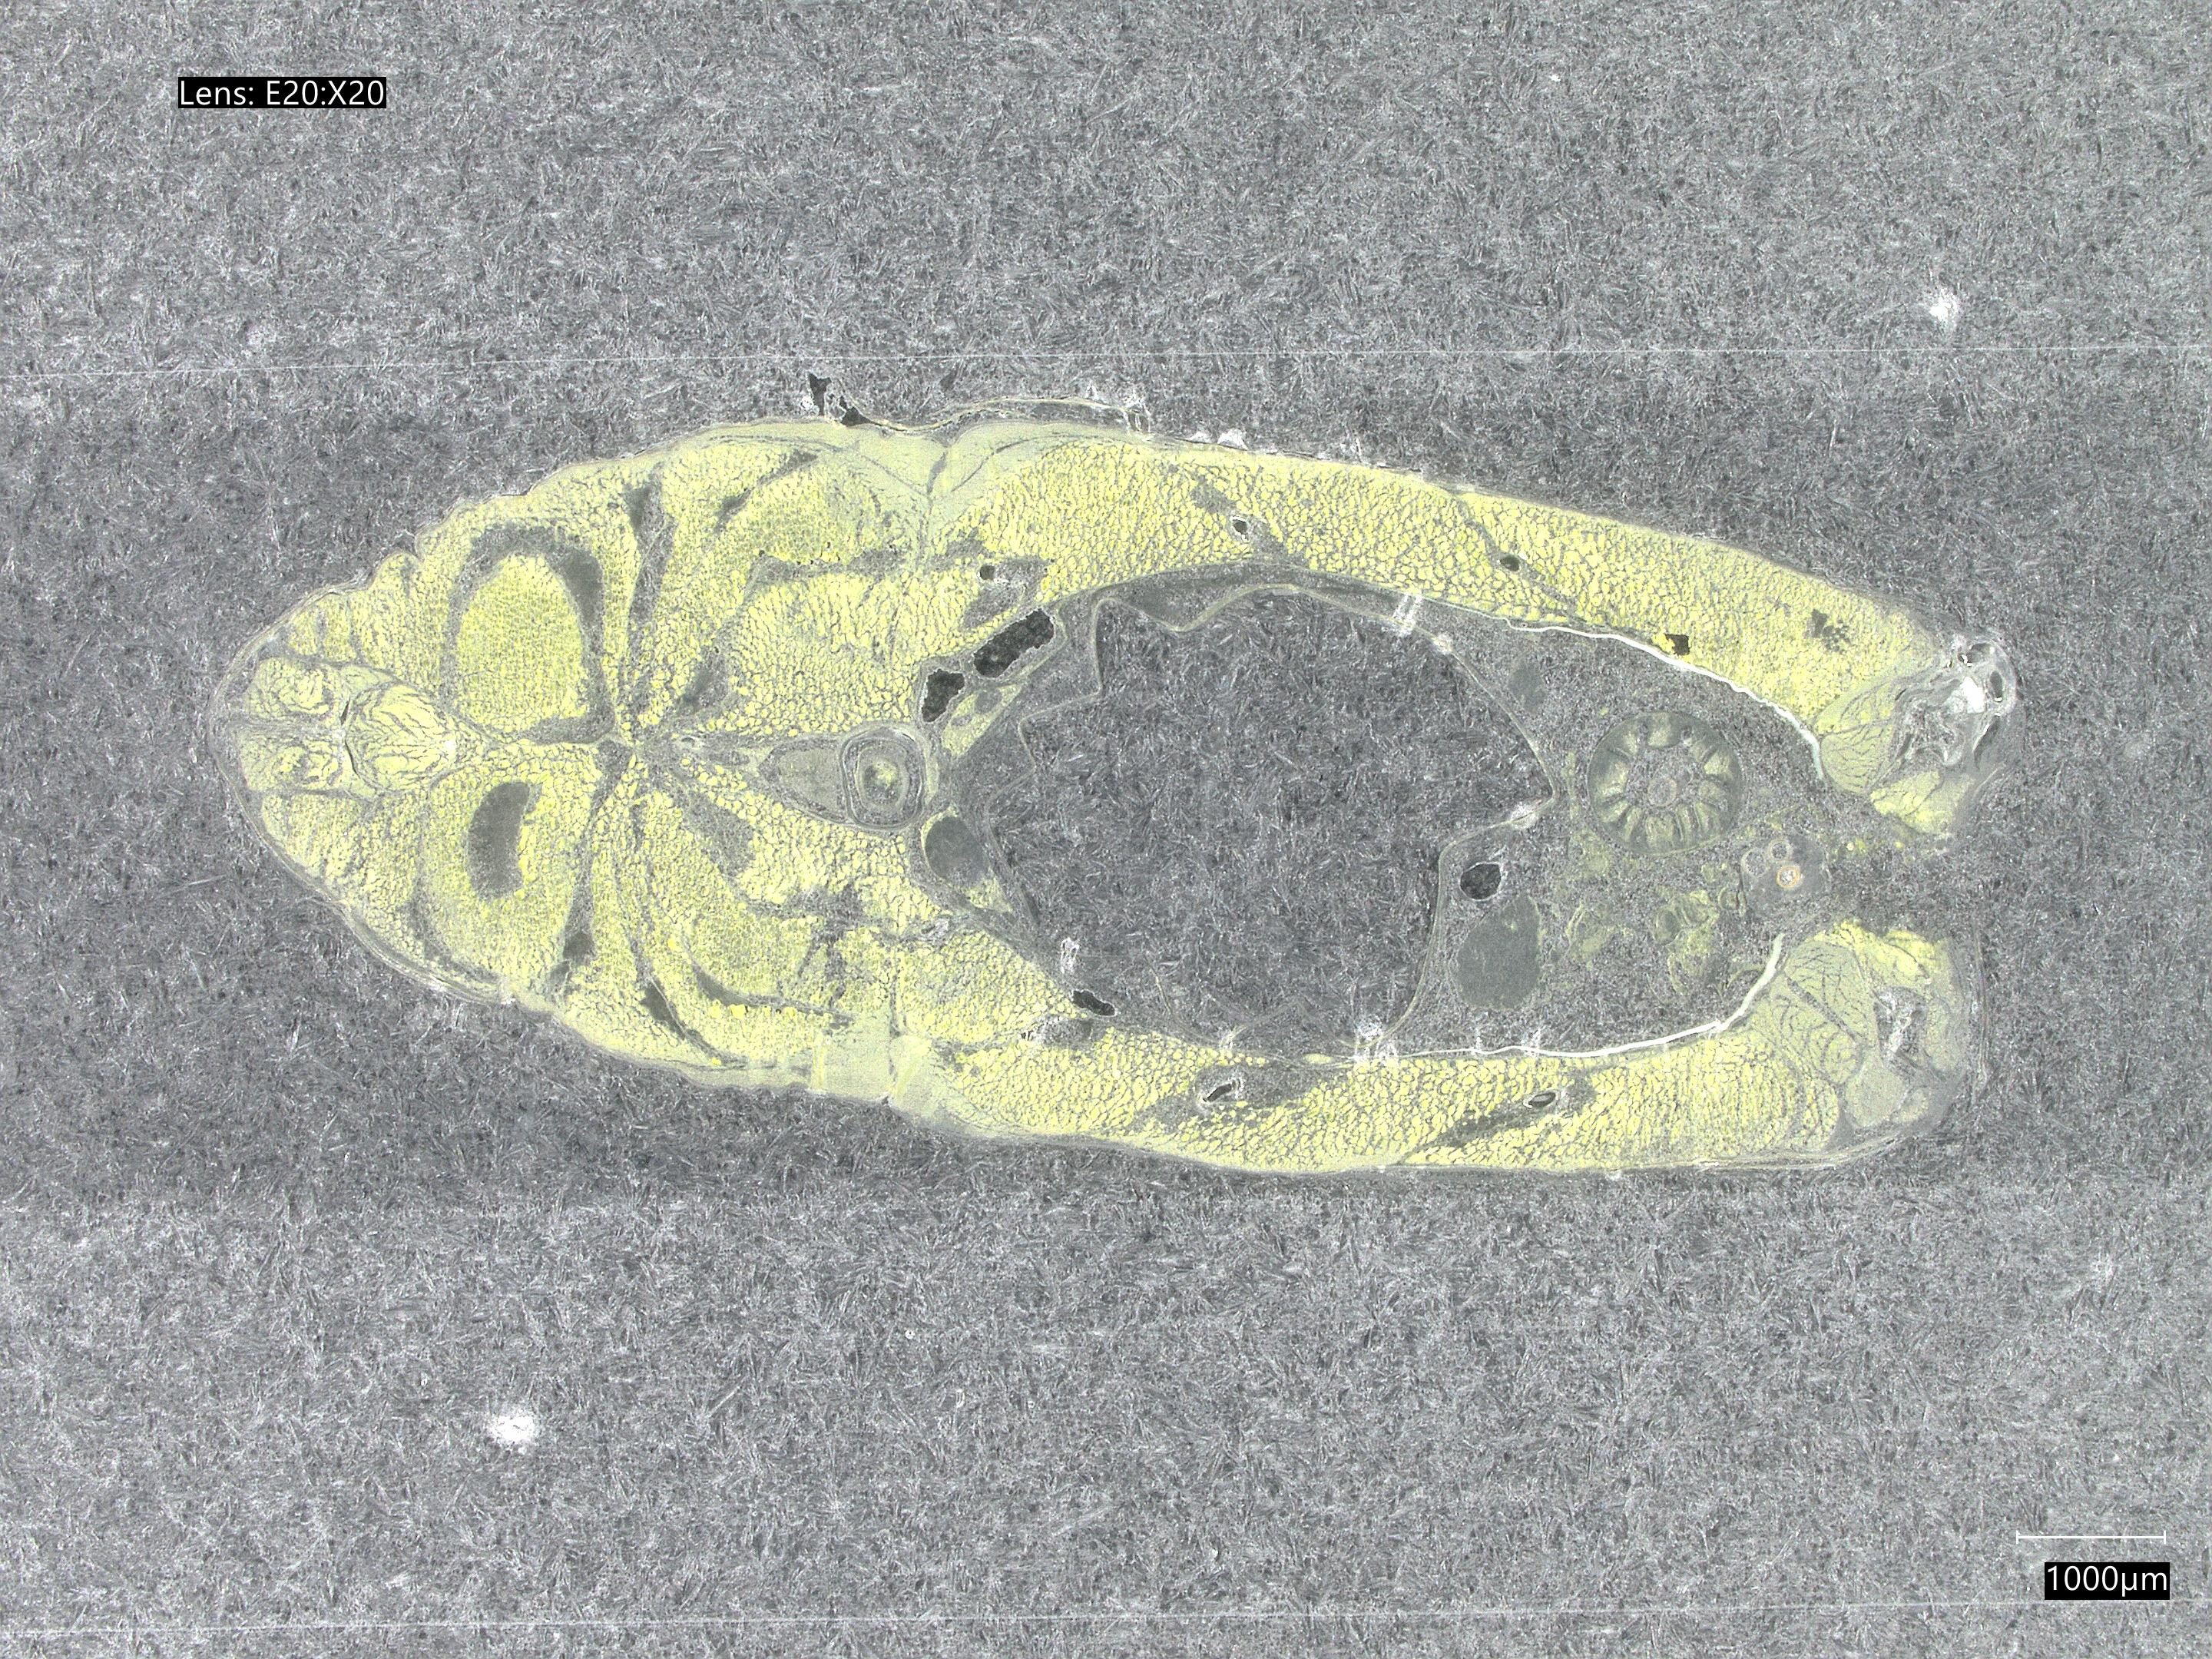
\includegraphics[width=\textwidth]{./fig/sample_1/normal.jpg}
        \caption{normal}
        \label{fig:normal}
    \end{minipage}
\end{figure}


对于每一张图片,我们需要将其标注为以上五个类别中的一个。这将作为我们的数据集,用于训练模型。


\FloatBarrier

\subsection{模型1:原始图像+简单的cnn网络}

对于一个全新的数据集,在不确定图像复杂度对应的何种模型之前,
首先尝试一个简单的cnn网络(架构如下),以了解数据集的特点和图像复杂度。

\begin{table}
\centering
\caption{Configuration of the simple CNN model}
\begin{tabular}{ccccc}
    \toprule
    \textbf{Layer Type} & \textbf{Configuration a} & \textbf{Configuration b} & \textbf{Configuration c} \\
    \midrule
    Input Layer & - & - & - \\
    Conv Layer 1 & Conv3-32 (relu) & Conv3-16 (relu) & Conv3-32 (relu) \\
    Pooling Layer 1 & MaxPooling & MaxPooling& MaxPooling \\
    Conv Layer 2 & Conv3-32 (relu) & Conv3-32 (relu) & Conv3-32 (relu) \\
    Pooling Layer 2 & MaxPooling & MaxPooling& MaxPooling \\
    Conv Layer 3 & Conv3-32 (relu) & Conv3-64 (relu) & Conv3-32 (relu) \\
    Pooling Layer 3 & MaxPooling & MaxPooling& MaxPooling \\
    Flattening Layer & Flatten() & Flatten() & Flatten() \\
    FC(Full connect) & Dense(128, relu) & Dense(128, relu) & Dense(256, relu) \\
    Output Layer & - & - & - \\
    \bottomrule
\end{tabular}
\label{tab:cnn_configuration}
\end{table}

\autoref{tab:cnn_configuration}显示的三个初始模型,分别为a,b,c。这三个模型的区别在于卷积层的数量和大小,全连接层的大小。a和b相比修改了卷积层的神经元数量,c相比a修改了全连接层的神经元数量。

数据的预处理部分,先将数据集分为训练集和测试集,其中训练集占80\%,测试集占20\%。之后将图像的长宽缩小一倍(即从2880*2160->1440*1080)并归一化数据。在训练过程中,我们使用了Adam优化器,交叉熵损失函数,使用早停。

下面图组展示了模型1a,1b,1c的准确度和损失随着训练次数的变化。

\begin{figure}
    \centering
    \begin{minipage}{0.45\textwidth}
        \centering
        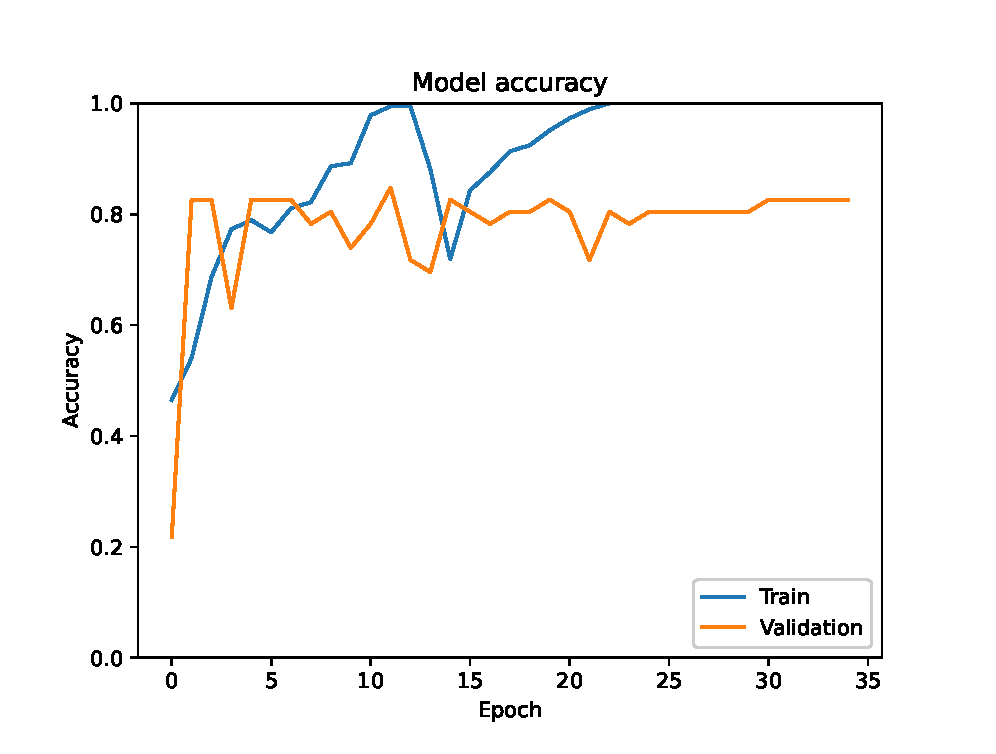
\includegraphics[width=\textwidth]{./fig/accuracy1a.eps}
        \caption{Model-1a accuracy}
        \label{fig:model1_acc}
    \end{minipage}
    \begin{minipage}{0.45\textwidth}
        \centering
        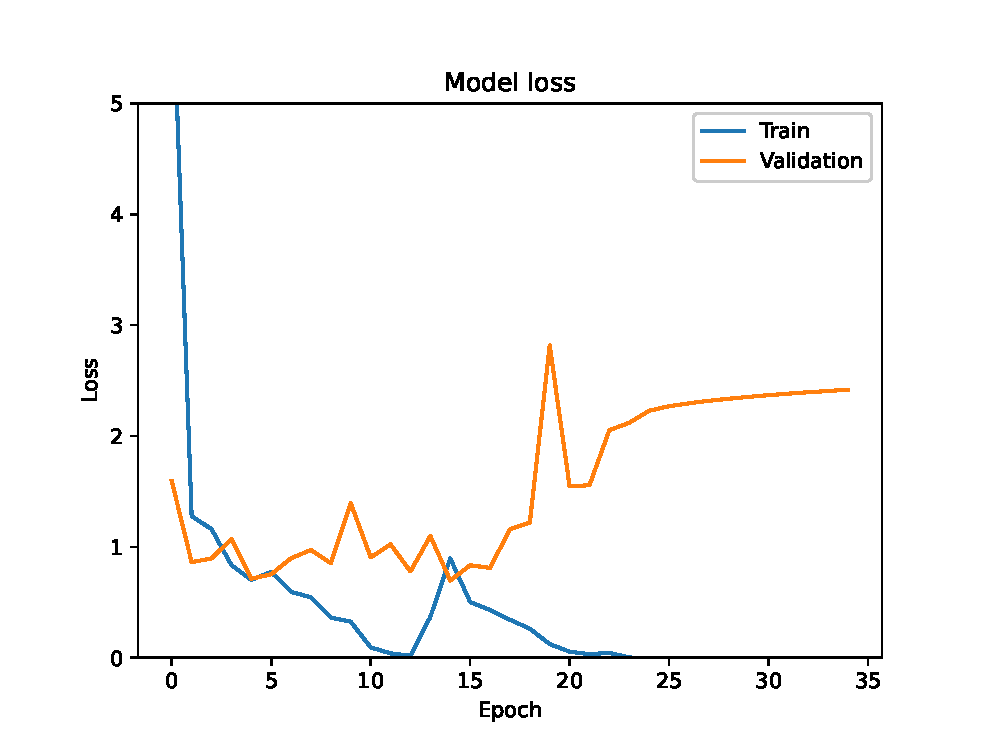
\includegraphics[width=\textwidth]{./fig/loss1a.eps}
        \caption{Model-1a loss}
        \label{fig:model1_loss}
    \end{minipage}
\end{figure}

\begin{figure}
    \centering
    \begin{minipage}{0.45\textwidth}
        \centering
        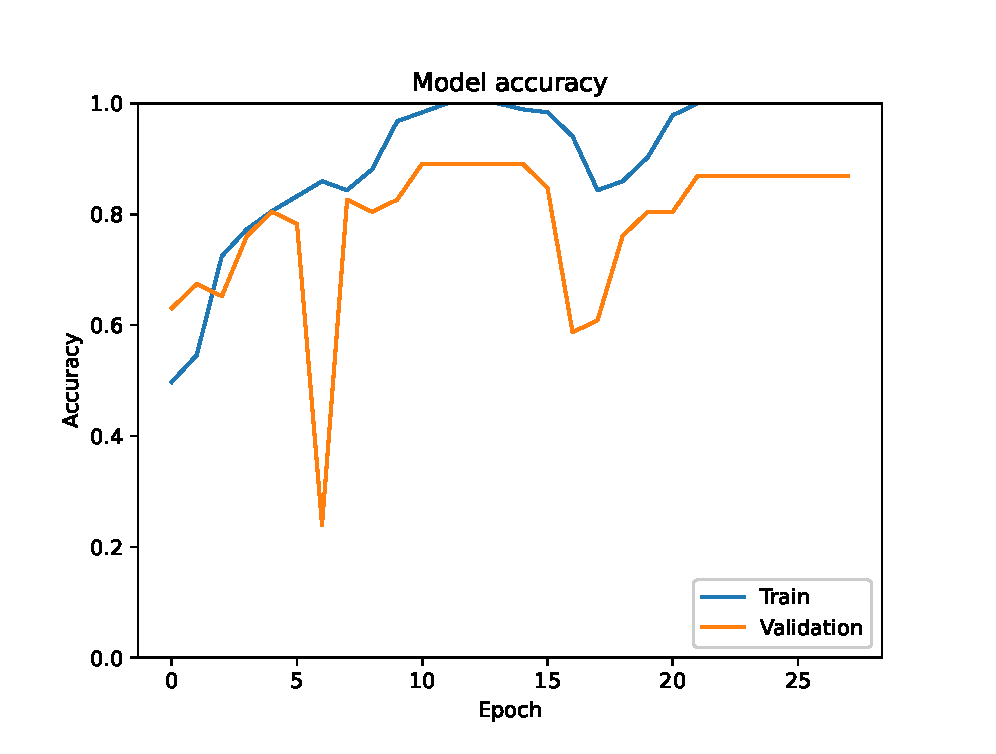
\includegraphics[width=\textwidth]{./fig/accuracy1b.eps}
        \caption{Model-1b accuracy}
        \label{fig:model1_acc}
    \end{minipage}
    \begin{minipage}{0.45\textwidth}
        \centering
        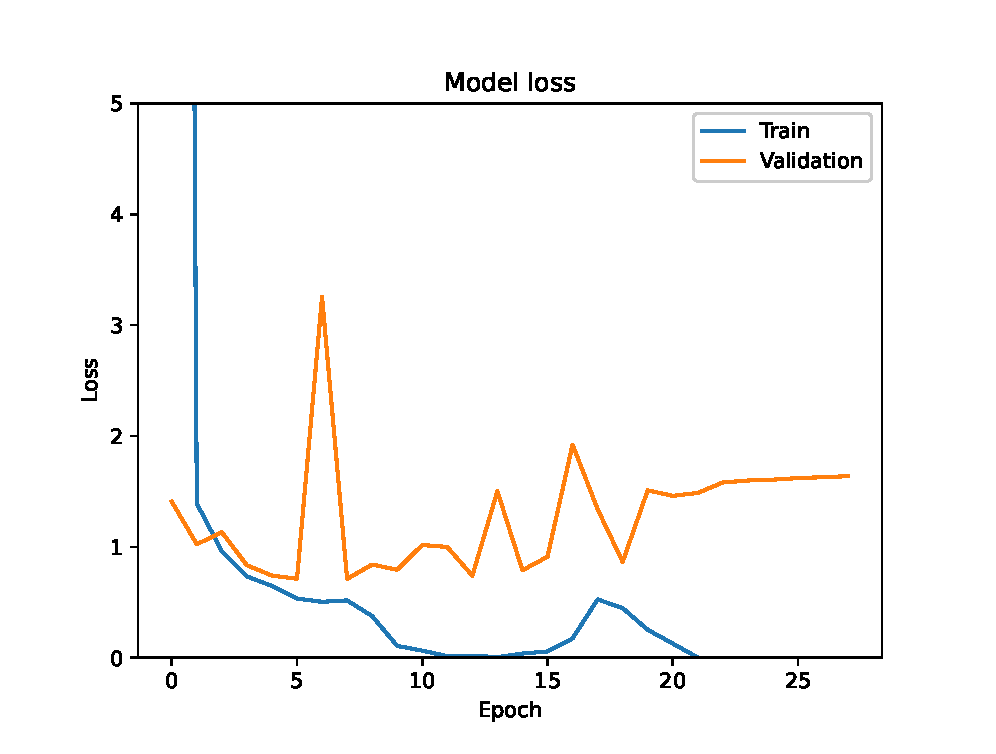
\includegraphics[width=\textwidth]{./fig/loss1b.eps}
        \caption{Model-1b loss}
        \label{fig:model1_loss}
    \end{minipage}
\end{figure}

\begin{figure}
    \centering
    \begin{minipage}{0.45\textwidth}
        \centering
        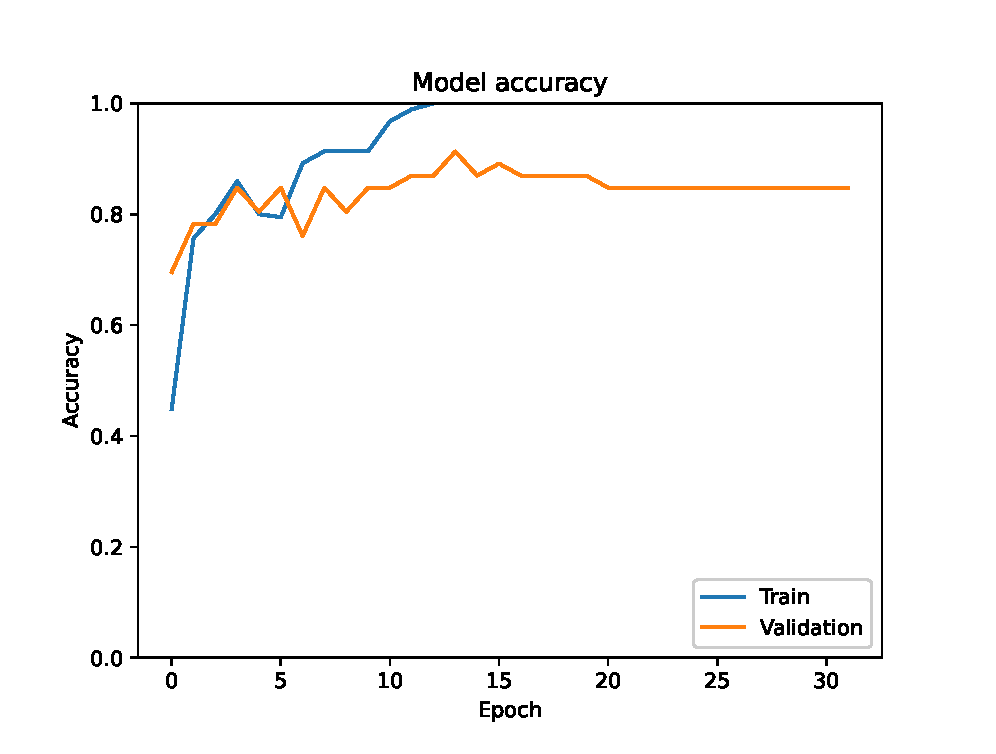
\includegraphics[width=\textwidth]{./fig/accuracy1c.eps}
        \caption{Model-1c accuracy}
        \label{fig:model1_acc}
    \end{minipage}
    \begin{minipage}{0.45\textwidth}
        \centering
        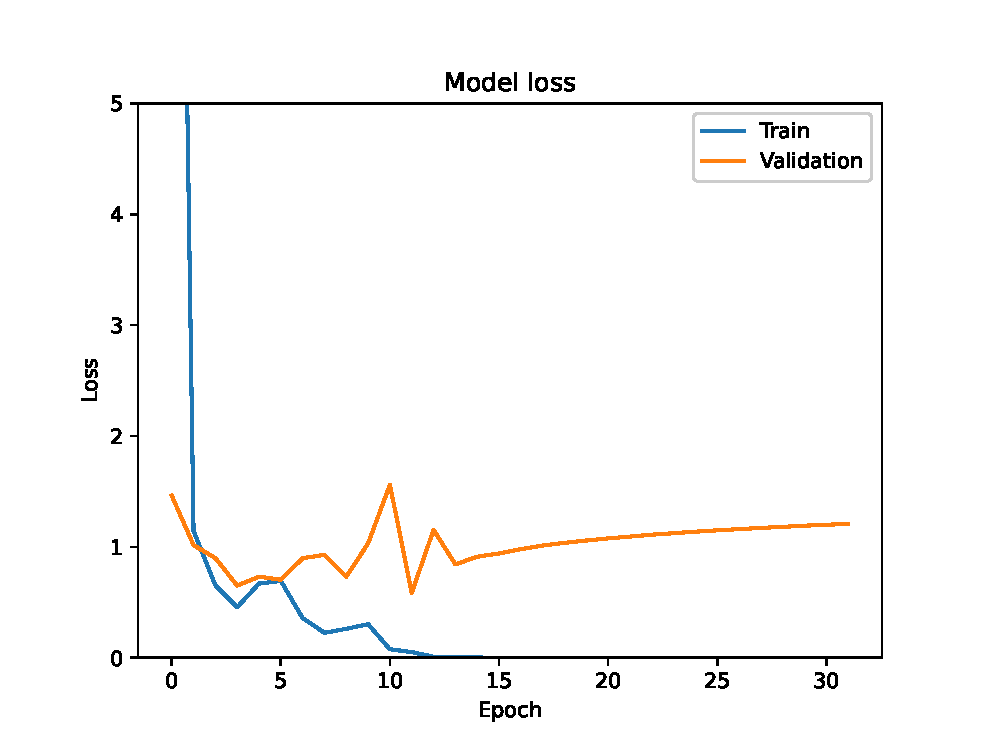
\includegraphics[width=\textwidth]{./fig/loss1c.eps}
        \caption{Model-1c loss}
        \label{fig:model1_loss}
    \end{minipage}
\end{figure}

观察到模型1a,1b,1c的准确度和损失随着训练次数的变化,发现三个模型的训练准确度和损失都在不断趋于1和0,反应了模型的训练效果良好。但是在测试集上的准确度则是收敛于0.8-0.85左右,损失则收敛于大于1的值(模型1a甚至趋于2.5)。这说明模型在训练集上表现良好,但是在测试集上表现欠佳。这可能和数据量过小,模型过于简单(图像过于复杂)有关。可见模型不能很好的泛化到验证集上。


%具体的测试集测试在第五章




\subsection{改进:图片预处理}

\subsection{模型2:预处理图像+简单的cnn网络}

\subsection{模型3:原始图像+迁移学习}